% !TeX root = main.tex
\chapter{Evaluation}
\label{chap:evaluation}

\providecommand{\evalqanchor}[1]{\hypertarget{eval:#1}{\textbf{#1}}}
\providecommand{\evalqref}[1]{\hyperlink{eval:#1}{\textbf{#1}}}

This chapter uses \texttt{fedctl} to evaluate heterogeneous FL methods under real hardware and network effects rather than abstract delay or capacity models. The evaluation considers three complementary axes. First, compute heterogeneity asks whether weaker devices should train smaller subnetworks. Second, straggler-induced heterogeneity asks whether asynchronous coordination reduces time-to-target, defined as the elapsed wall-clock time required to reach a fixed validation-accuracy threshold, when clients return updates at uneven rates. Third, asynchronous submodel FL combines both forms of heterogeneity by studying asynchronous aggregation over heterogeneous submodel updates.

The chapter is organised around nine evaluation objectives:

\begin{enumerate}[leftmargin=*]
  \item \textbf{Compute heterogeneity.}
  \begin{itemize}[leftmargin=1.5em, nosep]
    \item \evalqanchor{C1}: Motivation for submodel FL under real-world heterogeneity.
    \item \evalqanchor{C2}: Quality, runtime, and bottlenecks of submodel FL on mixed devices.
    \item \evalqanchor{C3}: Client-side quality of trained submodels.
    \item \evalqanchor{C4}: Sensitivity to the client-capability mix.
  \end{itemize}
  \item \textbf{Straggler-induced heterogeneity.}
  \begin{itemize}[leftmargin=1.5em, nosep]
    \item \evalqanchor{S1}: Behaviour of asynchronous FL across data and device heterogeneity.
    \item \evalqanchor{S2}: Speed and slow-device representation under network perturbations.
    \item \evalqanchor{S3}: Stale-aware weighting under device-correlated skew.
  \end{itemize}
  \item \textbf{Asynchronous submodel FL.}
  \begin{itemize}[leftmargin=1.5em, nosep]
    \item \evalqanchor{A1}: Feasibility of asynchronous submodel FL across tasks and data regimes.
    \item \evalqanchor{A2}: Coverage-aware aggregation with \texttt{FedCover}.
  \end{itemize}
\end{enumerate}

% The first two sections isolate the method families before combining them. The compute-heterogeneity section evaluates the quality--speed and client-side submodel trade-offs of \texttt{HeteroFL}, \texttt{FedRolex}, and \texttt{FIARSE}. The straggler-induced heterogeneity section evaluates \texttt{FedAsync}, \texttt{FedBuff}, and \texttt{FedStaleWeight} as standard asynchronous baselines, using client trips, wall-clock time, staleness, update share, and aggregate weight share to separate speed from representation. The final section then evaluates \texttt{FedCover}. This makes the chapter's contribution two-level: it first measures asynchronous submodel FL, then tests the proposed coverage correction designed specifically for that setting.

\FloatBarrier
\section{Compute Heterogeneity}
\label{sec:eval_compute_heterogeneity}

Compute heterogeneity changes both what a client can train and what comparison is meaningful: smaller submodels may reduce wall-clock cost, but can also change global accuracy and client-side model quality. Original submodel-FL evaluations mainly report accuracy with model-size, FLOP, or storage proxies; the cluster runs here add measured wall-clock time, client timing, and local submodel quality on real edge devices. Building on the heterogeneity in Section~\ref{sec:background_compute_heterogeneity} and the submodel FL methods reviewed in Section~\ref{sec:related_model_heterogeneous_fl}, this section evaluates \texttt{HeteroFL}, \texttt{FedRolex}, and \texttt{FIARSE}. The evaluation first motivates reduced-rate participation with a weak-client inclusion decision, then measures submodel-FL quality, runtime, and bottlenecks, client-side submodel quality, and sensitivity to the client-capability mix.

\FloatBarrier
\subsection{Weak-Client Inclusion Decision}

\paragraph{Setup.}
Reflecting edge deployments where lower-capability devices may be more numerous than high-performance clients, the experiment models \(15\) logical clients: \(5\) placed on stronger \texttt{rpi5} devices and \(10\) placed on weaker \texttt{rpi4} devices, with non-IID data assigned to every client. This subsection addresses \evalqref{C1}: the deployment trade-off between excluding the weaker majority, training those clients with full models, or including them through reduced-capacity submodels. This choice affects both runtime and whether clients placed on weaker devices can feasibly train the assigned model. A useful method should therefore \textbf{retain the weak clients' data while avoiding the synchronous-round cost and memory pressure of full-model training}.
\begin{figure}[!htbp]
\centering
\begin{tikzpicture}[
  labstrong/.style={circle, draw=paletteGreen!80!black, fill=paletteGreen!13, minimum size=6.2mm, inner sep=0pt},
  labweak/.style={circle, draw=paletteOrange!95!black, fill=paletteOrange!18, minimum size=6.2mm, inner sep=0pt},
  decision/.style={rounded corners=2pt, draw=black!35, fill=gray!4, align=center, text width=3.95cm, minimum height=2.65cm, inner sep=3pt, font=\small},
  arrow/.style={-Latex, line width=0.65pt, draw=black!55},
]
\node[font=\bfseries] at (0, 3) {Realistic non-IID deployment};
\node[align=center, font=\small, text width=7.4cm] at (0, 2.15) {\(15\) clients hold valuable local data, but weaker-device clients are the majority.};

\foreach \x/\y in {-3.45/1.2,-2.75/1.20,-2.05/1.20,-1.35/1.20,-0.65/1.20} {
  \node[labstrong] at (\x,\y) {};
}
\foreach \x/\y in {0.65/1.20,1.35/1.20,2.05/1.20,2.75/1.20,3.45/1.20,0.65/0.55,1.35/0.55,2.05/0.55,2.75/0.55,3.45/0.55} {
  \node[labweak] at (\x,\y) {};
}
\node[font=\footnotesize, align=center] at (0,-0.05) {\textcolor{paletteGreen!70!black}{\(5\) stronger-device clients} \quad+\quad \textcolor{paletteOrange!90!black}{\(10\) weaker-device clients}};

\coordinate (split) at (0,-0.45);
\node[decision] (exclude) at (-4.5,-3) {\textbf{A: Exclude}\\weak clients\\[0.2em]\(5/15\) data\\[0.2em]\footnotesize fastest, but loses non-IID coverage};
\node[decision] (full) at (0,-3) {\textbf{B: Full inclusion}\\all clients rate \(1.0\)\\[0.2em]\(15/15\) data\\[0.2em]\footnotesize direct baseline, but often infeasible};
\node[decision, text width=4.55cm] (submodel) at (4.65,-3) {\textbf{C--E: Submodel}\\\textbf{inclusion}\\weak clients rate \(1/8\)\\[0.2em]\(15/15\) data\\[0.2em]\footnotesize practical inclusion path};

\draw[arrow] (split) -- (exclude.north);
\draw[arrow] (split) -- (full.north);
\draw[arrow] (split) -- (submodel.north);
\end{tikzpicture}
% Notes: the schematic abstracts a 15-client non-IID deployment where 5 clients are placed on stronger devices and 10 weaker-device clients still hold valuable data.
% The ablation compares excluding weak clients, full-model inclusion, and reduced-rate inclusion.
\caption{\textbf{Deployment decision behind the slow-client inclusion ablation.}}
\label{fig:compute_slow_majority_scenario}
\end{figure}

Figure~\ref{fig:compute_slow_majority_scenario} summarises the deployment choice. The CIFAR-10 non-IID experiment uses \(20\) server rounds, \(3\) local epochs, and a shared \(15\)-partition data universe. Case~A excludes the ten weaker-device clients and trains only on the five \texttt{rpi5} partitions. Cases~B--E use all clients: full-model \texttt{FedAvg} trains everyone at rate \(1.0\), while \texttt{HeteroFL}, \texttt{FedRolex}, and \texttt{FIARSE} assign the ten \texttt{rpi4} clients rate \(1/8\). Case~B shows the full-model alternative, where weak clients keep all data but must train the full model.

\definecolor{slowcaseA}{HTML}{0C5DA5}
\definecolor{slowcaseB}{HTML}{00B945}
\definecolor{slowcaseC}{HTML}{FF9500}
\definecolor{slowcaseD}{HTML}{FF2C00}
\definecolor{slowcaseE}{HTML}{845B97}

\begin{table}[!htbp]
\centering
\footnotesize
% Notes: all runs use 20 server rounds and 3 local epochs.
% Values are mean +/- one standard deviation over seeds 1337--1339.
% Accuracy is centralized test accuracy in percent.
% Runtime is end-to-end server runtime; Mean train round is mean logged synchronous train-round duration.
\caption{\textbf{Slow-client inclusion trade-off on CIFAR-10 (non-IID).} Values are mean \(\pm\) standard deviation over three seeds; runtime is end-to-end server time.}
\label{tab:compute_slow_majority}
\begin{adjustbox}{max width=\textwidth}
\begin{tabular}{cllccrrr}
\toprule
Case & Clients & Method & Data used & \texttt{rpi4} rate & Accuracy & \makecell{Runtime\\(min)} & \makecell{Mean train\\round (s)} \\
\midrule
\textcolor{slowcaseA}{\textbf{A}} & \(5\) \texttt{rpi5} & \texttt{FedAvg}   & \(5/15\) & excluded & \(63.59\pm2.69\) & \(38.8\pm3.9\)   & \(76.1\pm11.5\)   \\
\textcolor{slowcaseB}{\textbf{B}} & \(5\) \texttt{rpi5}+\(10\) \texttt{rpi4} & \texttt{FedAvg}   & \(15/15\) & \(1.0\)  & \(73.12\pm0.95\) & \(137.5\pm8.5\) & \(373.4\pm17.5\) \\
\textcolor{slowcaseC}{\textbf{C}} & \(5\) \texttt{rpi5}+\(10\) \texttt{rpi4} & \texttt{HeteroFL} & \(15/15\) & \(1/8\)  & \evalsecond{\(64.30\pm2.35\)} & \evalbest{\(56.5\pm15.2\)}  & \(125.9\pm25.6\)   \\
\textcolor{slowcaseD}{\textbf{D}} & \(5\) \texttt{rpi5}+\(10\) \texttt{rpi4} & \texttt{FedRolex} & \(15/15\) & \(1/8\)  & \(62.74\pm2.87\) & \evalsecond{\(60.8\pm17.6\)}  & \(127.8\pm29.5\)   \\
\textcolor{slowcaseE}{\textbf{E}} & \(5\) \texttt{rpi5}+\(10\) \texttt{rpi4} & \texttt{FIARSE}   & \(15/15\) & \(1/8\)  & \evalbest{\(67.83\pm1.71\)} & \(155.1\pm14.9\) & \(425.2\pm32.9\) \\
\bottomrule
\end{tabular}
\end{adjustbox}
\par\vspace{0.5em}
{\centering\scriptsize \textcolor{evalBestText}{\textbf{Red bold}} text marks the \textbf{best} value and \textcolor{evalSecondText}{blue} text the \textbf{second-best} value among comparable entries.\par}
\end{table}

\paragraph{Interpretation.}
Table~\ref{tab:compute_slow_majority} makes the trade-off explicit. Case~A is fastest at \(38.8\) minutes because it trains only on the strong-device partitions, but it uses only \(5/15\) partitions and stops nearly ten percentage points below full-model inclusion. Case~B gives the highest final accuracy at \(73.12\%\), but is slowest at \(137.5\) minutes and can be impractical on weak devices because full-model training needs more memory. Reduced-rate inclusion is the practical middle ground: \texttt{HeteroFL} and \texttt{FedRolex} keep all partitions while finishing in \(56\)--\(61\) minutes, and \texttt{FIARSE} gives the best reduced-rate accuracy at \(67.83\%\). Its sparse masks are executed by dense PyTorch kernels in this deployment, however, so testing the paper's wall-clock efficiency argument would require sparse kernels or hardware-supported sparse execution.

% \begin{figure}[!htbp]
% \centering
% 
\includegraphics[width=0.98\textwidth]{figures/compute_slow_majority_tradeoff.pdf}
% % Notes: curves report across-seed mean centralized CIFAR-10 test accuracy against mean wall-clock time.
% % Shaded bands denote +/- one standard deviation over seeds 1337--1339.
% % Case A excludes the ten rpi4 partitions; Case B includes all data with full rpi4 models; Cases C--E use all data with reduced rpi4 rates.
% \caption{\textbf{Accuracy--time trade-off for slow-client inclusion.}}
% \label{fig:compute_slow_majority_tradeoff}
% \end{figure}

\paragraph{Takeaways.}
\begin{itemize}[leftmargin=*, nosep]
  \item Excluding slow clients is fastest, but it discards \(10/15\) non-IID partitions and loses almost \(10\) percentage points against full inclusion.
  \item Full-model inclusion gives the best final accuracy, \(73.12\%\), but costs \(137.5\) minutes and can be impractical for weak devices due to memory constraints.
  \item Reduced-rate inclusion is the practical middle ground: \texttt{HeteroFL} and \texttt{FedRolex} retain all partitions and finish in about \(1\) hour, while \texttt{FIARSE} gives stronger reduced-rate accuracy without realised sparse-kernel speedup.
\end{itemize}

\FloatBarrier
\subsection{Submodel FL on Mixed Devices: Quality and Runtime}

\paragraph{Setup.}
The previous subsection showed why reduced-rate inclusion is the relevant deployment choice: excluding weak clients loses data, while full-model inclusion is slow and can exceed weak-device memory budgets. This subsection addresses \evalqref{C2} by asking whether that choice remains useful beyond the motivating CIFAR-10 case. It sweeps \texttt{HeteroFL}, \texttt{FedRolex}, and \texttt{FIARSE} across tasks and data regimes on a mixed \texttt{rpi4}/\texttt{rpi5} testbed, measuring global quality, client-side submodel quality, end-to-end runtime, and client-level bottlenecks.

The benchmark uses a \(20\)-node mixed-device testbed, \(10\times\texttt{rpi4}+10\times\texttt{rpi5}\), for California Housing, Fashion-MNIST, and CIFAR-10. Appendix~\ref{appendix:evaluation_tasks} describes these datasets and task models; using a fixed testbed keeps cross-task comparisons consistent.

Submodel clients receive one of four model rates, \(0.125,0.25,0.5,1.0\), where the rate is the fraction of the full trainable parameter budget available locally. As shown in Figure~\ref{fig:compute_model_rate_assignment}, smaller rates are assigned to \texttt{rpi4} clients and larger rates to \texttt{rpi5} clients, with \(5\) clients in each group. The remaining run settings are listed in Appendix~\ref{appendix:evaluation_settings}.

The main metrics are client-side submodel quality, end-to-end runtime, and client-level timing. California Housing is a light-workload control where orchestration and evaluation should dominate; Fashion-MNIST is a smaller image task; CIFAR-10 is the most compute-bound workload and should benefit most from model-rate reduction.


\begin{figure}[!htbp]
\centering
\begin{tikzpicture}[
  font=\small,
  fullmodel/.style={draw=black!45, line width=0.45pt, fill=white},
  active/.style={draw=paletteGreen!80!black, line width=0.5pt, fill=paletteGreen!28},
  device/.style={draw=black!35, rounded corners=2pt, fill=black!4, align=center, minimum height=0.65cm},
  note/.style={font=\footnotesize, align=center, text=black!70}
]
\def\fullside{1.45}
\newcommand{\ratecard}[5]{%
  \begin{scope}[shift={(#1,0)}]
    \node[font=\footnotesize\bfseries] at (0.725,2.08) {#2};
    \draw[fullmodel] (0,0.42) rectangle ++(\fullside,\fullside);
    \draw[active] (0,0.42) rectangle ++(#3,#3);
    \node[note] at (0.725,0.08) {#4};
    \node[note] at (0.725,-0.28) {#5};
  \end{scope}
}
\ratecard{0.0}{rate \(0.125\)}{0.51}{\(5\) clients}{\texttt{rpi4}}
\ratecard{1.9}{rate \(0.25\)}{0.73}{\(5\) clients}{\texttt{rpi4}}
\ratecard{4.3}{rate \(0.5\)}{1.03}{\(5\) clients}{\texttt{rpi5}}
\ratecard{6.2}{rate \(1.0\)}{1.45}{\(5\) clients}{\texttt{rpi5}}

\node[device, minimum width=2.8cm] at (1.68,-0.95) {\texttt{rpi4}: smaller rates};
\node[device, minimum width=2.8cm] at (5.98,-0.95) {\texttt{rpi5}: larger rates};
\draw[-{Latex[length=2.2mm]}, paletteGreen!80!black, line width=0.5pt] (1.68,-0.58) -- (1.68,-0.37);
\draw[-{Latex[length=2.2mm]}, paletteGreen!80!black, line width=0.5pt] (5.98,-0.58) -- (5.98,-0.37);
\node[note] at (3.83,2.45) {Shaded area is proportional to the configured parameter-budget fraction};
\end{tikzpicture}
\caption{\textbf{Device-aware model-rate assignment for the compute heterogeneous runs.} Each outline denotes the full model; shaded area denotes parameter-budget fraction.}
\label{fig:compute_model_rate_assignment}
\end{figure}


\begin{table}[H]
\centering
\scriptsize
\renewcommand{\arraystretch}{1.06}
\setlength{\tabcolsep}{2pt}
% Notes: both task blocks report mean +/- standard deviation over seeds 1337--1339.
% Local is the peak client-side evaluation score observed during training.
% Model(.) is the post-training score of the extracted submodel on the global test dataset.
% Global is the peak full-model score on the global test dataset.
% CIFAR-10 entries are accuracies; California Housing entries are R^2.
% Fashion-MNIST entries are accuracies.
% Blank cells denote pending experiments; dashes denote non-applicable method--metric combinations.
\caption{\textbf{Compute-heterogeneity results by task and data regime.} Local, submodel, and global scores are reported; image tasks use accuracy and California Housing uses \(R^2\).}
\label{tab:compute_main_results}
\begin{adjustbox}{max width=\textwidth} 
\begin{tabular}{@{}lllcccccc@{}}
\toprule
Task & Data & Method & Local & \makecell[c]{M (1/8)} & \makecell[c]{M (1/4)} & \makecell[c]{M (1/2)} & \makecell[c]{M (1.0)} & Global \\
\midrule
\multirow{8}{*}{\makecell[l]{California\\Housing}} & \multirow{4}{*}{IID} & \cellcolor{black!8}\texttt{FedAvg} & \cellcolor{black!8}0.723$\pm$0.001 & \cellcolor{black!8}-- & \cellcolor{black!8}-- & \cellcolor{black!8}-- & \cellcolor{black!8}-- & \cellcolor{black!8}0.724$\pm$0.001 \\
& & \texttt{HeteroFL} & \evalsecond{0.612$\pm$0.008} & \evalsecond{0.479$\pm$0.028} & \evalsecond{0.629$\pm$0.010} & \evalsecond{0.659$\pm$0.005} & \evalsecond{0.693$\pm$0.006} & \evalsecond{0.693$\pm$0.006} \\
& & \texttt{FedRolex} & 0.562$\pm$0.011 & 0.359$\pm$0.033 & 0.581$\pm$0.010 & 0.639$\pm$0.006 & 0.679$\pm$0.003 & 0.679$\pm$0.003 \\
& & \texttt{FIARSE} & \evalbest{0.688$\pm$0.002} & \evalbest{0.665$\pm$0.002} & \evalbest{0.686$\pm$0.006} & \evalbest{0.706$\pm$0.001} & \evalbest{0.710$\pm$0.002} & \evalbest{0.710$\pm$0.002} \\
\cmidrule(lr){2-9}
& \multirow{4}{*}{Non-IID} & \cellcolor{black!8}\texttt{FedAvg} & \cellcolor{black!8}0.654$\pm$0.024 & \cellcolor{black!8}-- & \cellcolor{black!8}-- & \cellcolor{black!8}-- & \cellcolor{black!8}-- & \cellcolor{black!8}0.711$\pm$0.007 \\
& & \texttt{HeteroFL} & \evalsecond{0.562$\pm$0.015} & \evalsecond{0.540$\pm$0.017} & \evalsecond{0.601$\pm$0.030} & \evalbest{0.657$\pm$0.023} & \evalbest{0.689$\pm$0.005} & \evalbest{0.689$\pm$0.005} \\
& & \texttt{FedRolex} & 0.404$\pm$0.039 & 0.242$\pm$0.096 & 0.482$\pm$0.027 & 0.514$\pm$0.027 & 0.597$\pm$0.017 & 0.597$\pm$0.017 \\
& & \texttt{FIARSE} & \evalbest{0.668$\pm$0.025} & \evalbest{0.621$\pm$0.008} & \evalbest{0.681$\pm$0.015} & \evalsecond{0.643$\pm$0.061} & \evalsecond{0.614$\pm$0.070} & \evalsecond{0.614$\pm$0.070} \\
\midrule
\multirow{8}{*}{CIFAR-10} & \multirow{4}{*}{IID} & \cellcolor{black!8}\texttt{FedAvg} & \cellcolor{black!8}77.43$\pm$0.13 & \cellcolor{black!8}-- & \cellcolor{black!8}-- & \cellcolor{black!8}-- & \cellcolor{black!8}-- & \cellcolor{black!8}79.38$\pm$0.25 \\
& & \texttt{HeteroFL} & \evalsecond{66.21$\pm$0.29} & \evalsecond{59.39$\pm$1.00} & \evalsecond{66.55$\pm$0.39} & \evalsecond{72.19$\pm$0.33} & \evalsecond{74.95$\pm$0.41} & \evalsecond{74.95$\pm$0.41} \\
& & \texttt{FedRolex} & 63.69$\pm$0.53 & 55.07$\pm$1.23 & 64.22$\pm$0.72 & 70.27$\pm$0.49 & 74.16$\pm$0.39 & 74.24$\pm$0.27 \\
& & \texttt{FIARSE} & \evalbest{71.65$\pm$6.30} & \evalbest{71.47$\pm$8.48} & \evalbest{73.28$\pm$8.00} & \evalbest{74.65$\pm$6.49} & \evalbest{76.43$\pm$2.08} & \evalbest{76.43$\pm$2.08} \\
\cmidrule(lr){2-9}
& \multirow{4}{*}{Non-IID} & \cellcolor{black!8}\texttt{FedAvg} & \cellcolor{black!8}69.02$\pm$0.44 & \cellcolor{black!8}-- & \cellcolor{black!8}-- & \cellcolor{black!8}-- & \cellcolor{black!8}-- & \cellcolor{black!8}75.93$\pm$0.67 \\
& & \texttt{HeteroFL} & \evalsecond{60.12$\pm$0.31} & \evalsecond{49.61$\pm$5.04} & \evalsecond{55.09$\pm$3.22} & 55.48$\pm$8.77 & 59.02$\pm$6.25 & 64.86$\pm$2.03 \\
& & \texttt{FedRolex} & 56.10$\pm$0.76 & 40.62$\pm$1.39 & 53.98$\pm$1.70 & \evalsecond{59.09$\pm$3.19} & \evalsecond{61.93$\pm$1.00} & \evalsecond{65.72$\pm$0.66} \\
& & \texttt{FIARSE} & \evalbest{64.57$\pm$2.56} & \evalbest{71.91$\pm$1.33} & \evalbest{70.85$\pm$0.47} & \evalbest{69.31$\pm$1.64} & \evalbest{69.43$\pm$1.54} & \evalbest{70.55$\pm$1.75} \\
\midrule
\multirow{8}{*}{\makecell[l]{Fashion\\MNIST}} & \multirow{4}{*}{IID} & \cellcolor{black!8}\texttt{FedAvg} & \cellcolor{black!8}82.84$\pm$0.20 & \cellcolor{black!8}-- & \cellcolor{black!8}-- & \cellcolor{black!8}-- & \cellcolor{black!8}-- & \cellcolor{black!8}83.88$\pm$0.15 \\
& & \texttt{HeteroFL} & \evalsecond{74.28$\pm$0.62} & \evalsecond{66.81$\pm$2.63} & \evalsecond{74.92$\pm$0.35} & \evalsecond{79.11$\pm$1.03} & \evalsecond{81.95$\pm$0.46} & \evalsecond{81.95$\pm$0.46} \\
& & \texttt{FedRolex} & 61.83$\pm$1.98 & 44.28$\pm$5.72 & 63.48$\pm$4.56 & 70.42$\pm$2.01 & 77.31$\pm$1.09 & 77.31$\pm$1.09 \\
& & \texttt{FIARSE} & \evalbest{81.95$\pm$0.43} & \evalbest{81.87$\pm$0.50} & \evalbest{83.01$\pm$0.16} & \evalbest{83.72$\pm$0.24} & \evalbest{83.57$\pm$0.20} & \evalbest{83.57$\pm$0.20} \\
\cmidrule(lr){2-9}
& \multirow{4}{*}{Non-IID} & \cellcolor{black!8}\texttt{FedAvg} & \cellcolor{black!8}76.95$\pm$1.66 & \cellcolor{black!8}-- & \cellcolor{black!8}-- & \cellcolor{black!8}-- & \cellcolor{black!8}-- & \cellcolor{black!8}80.86$\pm$3.00 \\
& & \texttt{HeteroFL} & \evalbest{69.10$\pm$6.53} & \evalsecond{51.28$\pm$4.59} & \evalsecond{67.03$\pm$3.01} & \evalsecond{70.09$\pm$5.96} & \evalsecond{69.73$\pm$4.73} & \evalsecond{69.73$\pm$4.73} \\
& & \texttt{FedRolex} & 51.18$\pm$15.45 & 37.74$\pm$5.90 & 55.10$\pm$4.66 & 59.74$\pm$8.27 & 64.13$\pm$6.89 & 64.13$\pm$6.89 \\
& & \texttt{FIARSE} & \evalsecond{68.09$\pm$3.62} & \evalbest{75.75$\pm$2.19} & \evalbest{75.91$\pm$3.05} & \evalbest{77.08$\pm$4.65} & \evalbest{76.38$\pm$4.04} & \evalbest{76.38$\pm$4.04} \\
\bottomrule
\end{tabular}
\end{adjustbox}
\par\vspace{0.5em}
{\centering\scriptsize \textcolor{evalBestText}{\textbf{Red bold}} text marks the \textbf{best} value and \textcolor{evalSecondText}{blue} text the \textbf{second-best} value among comparable entries.\par}
\end{table}


\begin{table}[H]
\centering
\scriptsize
\renewcommand{\arraystretch}{1.05}
\setlength{\tabcolsep}{2.9pt}
% Notes: entries report mean +/- standard deviation over seeds 1337--1339.
% Runtime is end-to-end server-observed training time from runtime/total_server_s.
% Training columns separate round-level synchronous latency from the client-reported local training distribution.
% Evaluation columns report synchronous client-evaluation and centralized server-evaluation latency.
% Lower is better for timing columns; lightly shaded rows denote the full-model FedAvg baseline.
\caption{\textbf{Compute-heterogeneity runtime and bottleneck decomposition.}}
\label{tab:compute_main_runtime}
\begin{adjustbox}{max width=\textwidth}
\begin{tabular}{@{}lllrrrrrr@{}}
\toprule
\multicolumn{3}{c}{\textbf{Setting}} &
\multicolumn{2}{c}{\textbf{End-to-end}} &
\multicolumn{2}{c}{\textbf{Training bottleneck}} &
\multicolumn{2}{c}{\textbf{Evaluation overhead}} \\
\cmidrule(lr){1-3}\cmidrule(lr){4-5}\cmidrule(lr){6-7}\cmidrule(l){8-9}
Task & Data & Method &
\makecell[c]{Runtime\\(min)} & Rel. &
\makecell[c]{Train\\round\\(s)} &
\makecell[c]{Client train\\\(\mu/\sigma\)\\(s)} &
\makecell[c]{Client\\eval\\(s)} &
\makecell[c]{Server\\eval\\(s)} \\
\midrule
\multirow{8}{*}{\makecell[l]{California\\Housing}}
& \multirow{4}{*}{IID}
& \cellcolor{black!5}\texttt{FedAvg} & \cellcolor{black!5}25.5$\pm$0.6 & \cellcolor{black!5}1.00$\times$ & \cellcolor{black!5}36.5$\pm$1.3 & \cellcolor{black!5}0.2 / 0.2 & \cellcolor{black!5}35.7$\pm$0.9 & \cellcolor{black!5}0.1$\pm$0.0 \\
& & \texttt{HeteroFL}  & \evalbest{25.6$\pm$1.8} & 1.00$\times$ & 36.3$\pm$1.0  & 0.2 / 0.1 & 35.9$\pm$1.2   & 0.1$\pm$0.0 \\
& & \texttt{FedRolex}  & \evalsecond{26.1$\pm$1.5} & 1.02$\times$ & 37.1$\pm$0.3  & 0.2 / 0.1 & 36.5$\pm$0.2   & 0.1$\pm$0.0 \\
& & \texttt{FIARSE}    & 26.2$\pm$1.4          & 1.03$\times$ & 37.5$\pm$0.0  & 0.3 / 0.3 & 36.3$\pm$0.1   & 0.1$\pm$0.0 \\
\cmidrule(lr){2-9}
& \multirow{4}{*}{Non-IID}
& \cellcolor{black!5}\texttt{FedAvg} & \cellcolor{black!5}37.0$\pm$0.7 & \cellcolor{black!5}1.00$\times$ & \cellcolor{black!5}26.7$\pm$2.7 & \cellcolor{black!5}0.2 / 0.2 & \cellcolor{black!5}26.8$\pm$2.2 & \cellcolor{black!5}0.1$\pm$0.0 \\
& & \texttt{HeteroFL}  & 38.5$\pm$3.0          & 1.04$\times$ & 28.5$\pm$1.7  & 0.2 / 0.1 & 27.0$\pm$0.9   & 0.1$\pm$0.0 \\
& & \texttt{FedRolex}  & \evalbest{37.4$\pm$2.1} & 1.01$\times$ & 26.0$\pm$2.1  & 0.2 / 0.1 & 27.8$\pm$0.8   & 0.1$\pm$0.0 \\
& & \texttt{FIARSE}    & \evalsecond{37.9$\pm$1.1} & 1.02$\times$ & 28.3$\pm$0.4  & 0.3 / 0.2 & 26.3$\pm$0.3   & 0.1$\pm$0.0 \\
\midrule
\multirow{8}{*}{\makecell[l]{Fashion\\MNIST}}
& \multirow{4}{*}{IID}
& \cellcolor{black!5}\texttt{FedAvg} & \cellcolor{black!5}37.8$\pm$1.2 & \cellcolor{black!5}1.19$\times$ & \cellcolor{black!5}65.8$\pm$0.5 & \cellcolor{black!5}12.5 / 9.6 & \cellcolor{black!5}36.4$\pm$0.1 & \cellcolor{black!5}6.5$\pm$0.1 \\
& & \texttt{HeteroFL}  & \evalsecond{31.9$\pm$0.3} & 1.00$\times$ & 50.1$\pm$1.0 & 7.1 / 4.4 & 35.3$\pm$0.1 & 6.7$\pm$0.0 \\
& & \texttt{FedRolex}  & \evalbest{31.8$\pm$0.4} & 1.00$\times$ & 50.4$\pm$0.9 & 7.2 / 4.6 & 34.8$\pm$0.4 & 6.7$\pm$0.1 \\
& & \texttt{FIARSE}    & 39.2$\pm$0.1 & 1.23$\times$ & 70.9$\pm$0.1 & 14.2 / 11.3 & 36.2$\pm$0.1 & 6.5$\pm$0.0 \\
\cmidrule(lr){2-9}
& \multirow{4}{*}{Non-IID}
& \cellcolor{black!5}\texttt{FedAvg} & \cellcolor{black!5}61.6$\pm$2.5 & \cellcolor{black!5}1.25$\times$ & \cellcolor{black!5}57.4$\pm$4.7 & \cellcolor{black!5}13.9 / 11.3 & \cellcolor{black!5}27.0$\pm$1.4 & \cellcolor{black!5}6.6$\pm$0.1 \\
& & \texttt{HeteroFL}  & \evalbest{49.2$\pm$3.3} & 1.00$\times$ & 38.9$\pm$4.2 & 7.7 / 5.4 & 26.3$\pm$1.1 & 6.6$\pm$0.1 \\
& & \texttt{FedRolex}  & \evalsecond{50.2$\pm$1.7} & 1.02$\times$ & 40.4$\pm$2.5 & 7.5 / 5.2 & 26.3$\pm$1.5 & 6.6$\pm$0.1 \\
& & \texttt{FIARSE}    & 65.7$\pm$3.5 & 1.34$\times$ & 63.1$\pm$6.0 & 15.9 / 13.2 & 26.6$\pm$0.9 & 6.6$\pm$0.1 \\
\midrule
\multirow{8}{*}{CIFAR-10}
& \multirow{4}{*}{IID}
& \cellcolor{black!5}\texttt{FedAvg} & \cellcolor{black!5}260.0$\pm$55.6 & \cellcolor{black!5}2.34$\times$ & \cellcolor{black!5}694.3$\pm$158.7 & \cellcolor{black!5}131.4 / 135.7 & \cellcolor{black!5}229.2$\pm$288.6 & \cellcolor{black!5}20.9$\pm$0.2 \\
& & \texttt{HeteroFL}  & \evalbest{111.1$\pm$11.7} & 1.00$\times$ & 252.9$\pm$37.4  & 59.6 / 47.4 & 119.6$\pm$118.9 & 21.5$\pm$0.2 \\
& & \texttt{FedRolex}  & \evalsecond{120.4$\pm$8.7} & 1.08$\times$ & 273.0$\pm$28.4  & 62.1 / 48.5 & 148.5$\pm$173.7 & 22.6$\pm$0.2 \\
& & \texttt{FIARSE}    & 208.6$\pm$81.5        & 1.88$\times$ & 539.5$\pm$242.7 & 127.2 / 115.3 & 335.3$\pm$277.0 & 22.1$\pm$0.9 \\
\cmidrule(lr){2-9}
& \multirow{4}{*}{Non-IID}
& \cellcolor{black!5}\texttt{FedAvg} & \cellcolor{black!5}305.9$\pm$24.7 & \cellcolor{black!5}2.27$\times$ & \cellcolor{black!5}392.4$\pm$35.4 & \cellcolor{black!5}125.5 / 107.1 & \cellcolor{black!5}176.8$\pm$236.8 & \cellcolor{black!5}22.8$\pm$0.4 \\
& & \texttt{HeteroFL}  & \evalsecond{148.6$\pm$10.1} & 1.10$\times$ & 157.7$\pm$15.3 & 47.0 / 34.5 & 195.9$\pm$15.8  & 23.2$\pm$1.3 \\
& & \texttt{FedRolex}  & \evalbest{135.0$\pm$10.8} & 1.00$\times$ & 139.8$\pm$16.6 & 43.3 / 29.7 & 175.5$\pm$15.9  & 22.9$\pm$1.2 \\
& & \texttt{FIARSE}    & 356.2$\pm$30.3        & 2.64$\times$ & 467.2$\pm$47.5 & 140.3 / 132.4 & 505.7$\pm$47.0  & 22.2$\pm$0.6 \\
\bottomrule
\end{tabular}
\end{adjustbox}
\par\vspace{0.2em}
{\centering\scriptsize Client train \(\mu/\sigma\) reports the average within-round client-training mean and standard deviation; other timing entries report mean \(\pm\) standard deviation over seeds.\par}
\end{table}


\paragraph{Interpretation.}
\texttt{FedAvg} remains the strongest full-model quality reference, reaching \(83.88\%\) on IID Fashion-MNIST, \(79.38\%\) on IID CIFAR-10, and \(R^2=0.724\) on IID California Housing. Among the heterogeneous methods, \texttt{FIARSE} gives the strongest image-task quality profile: on non-IID Fashion-MNIST it reaches \(76.38\%\) global accuracy, compared with \(69.73\%\) for \texttt{HeteroFL} and \(64.13\%\) for \texttt{FedRolex}; on non-IID CIFAR-10 it reaches \(70.55\%\), compared with \(64.86\%\) and \(65.72\%\). California Housing is the exception: under non-IID data, \texttt{HeteroFL} gives the strongest heterogeneous-method global score.



Runtime depends on task size. California Housing runtimes cluster around \(25\)--\(38\) minutes because sub-second local training is dominated by orchestration and evaluation. On Fashion-MNIST, \texttt{HeteroFL} and \texttt{FedRolex} reduce IID runtime from \(37.8\) minutes to about \(32\) minutes, and reduce non-IID runtime from \(61.6\) minutes to about \(50\) minutes. CIFAR-10 shows the largest compute-bound effect: \texttt{HeteroFL} and \texttt{FedRolex} reduce non-IID runtime from \(305.9\) minutes to \(148.6\) and \(135.0\) minutes. \texttt{FIARSE}'s quality result aligns with its paper motivation, but its dense PyTorch execution path prevents that quality advantage from becoming a wall-clock advantage here.

\begin{figure}[!htbp]
\centering
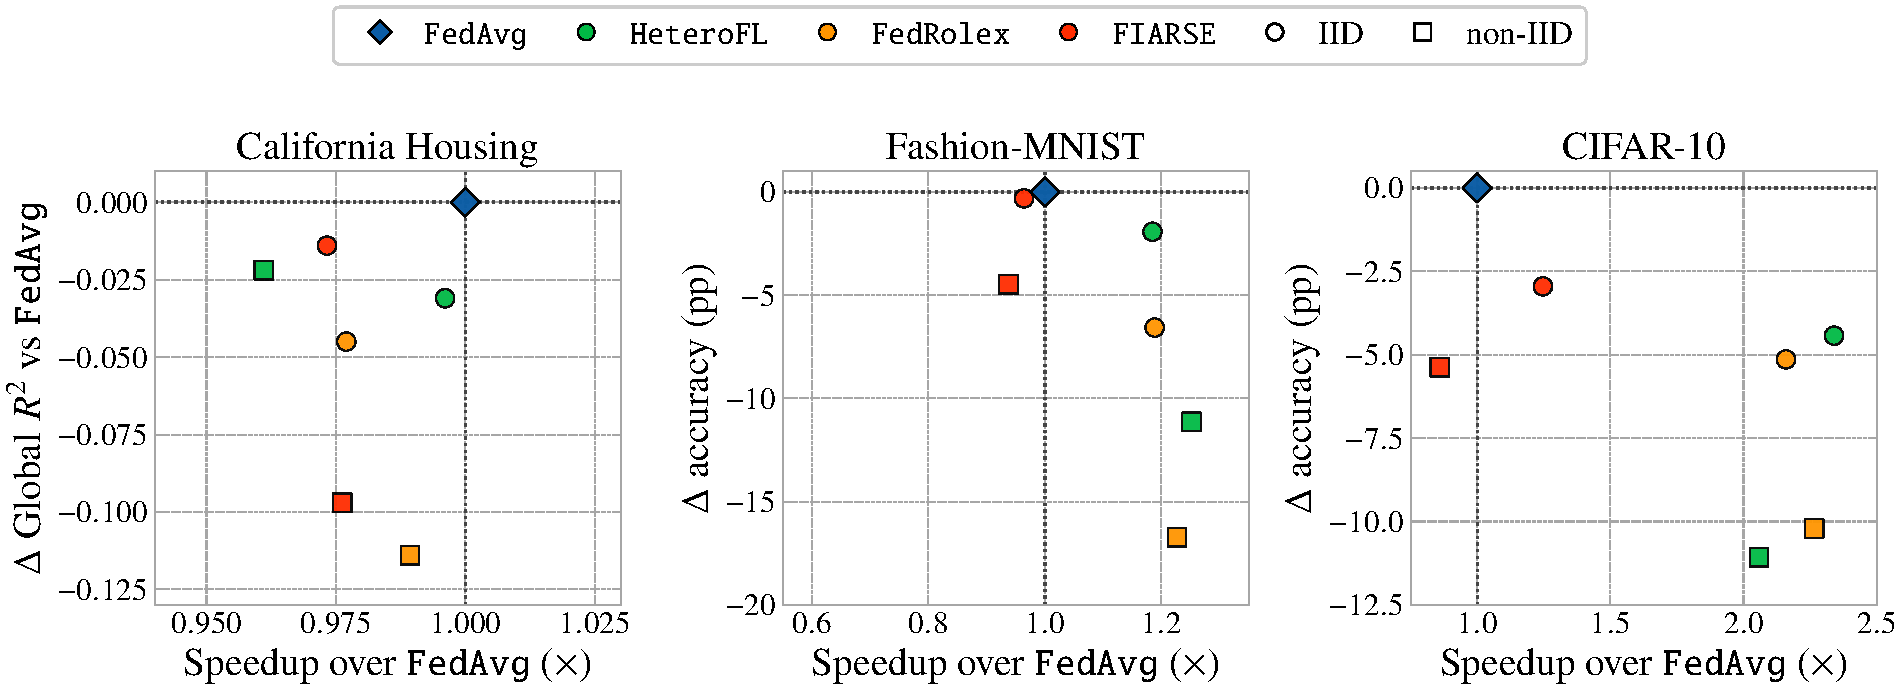
\includegraphics[width=0.95\textwidth]{figures/compute_main_quality_speed_tradeoff.pdf}
% Notes: points use mean global score and mean end-to-end runtime from Tables~\ref{tab:compute_main_results} and~\ref{tab:compute_main_runtime}.
% CIFAR-10 and Fashion-MNIST quality changes are percentage-point accuracy deltas; California Housing quality changes are raw R^2 deltas.
% The FedAvg diamond marks the reference point at 1x speedup and zero quality change in each task panel.
\caption{\textbf{Quality--speed trade-off relative to \texttt{FedAvg}.} Axes report wall-clock speedup and global-score change against the matching \texttt{FedAvg} baseline.}
% Non-baseline points compare a heterogeneous method against the matching \texttt{FedAvg} baseline for the same task and data regime; the \texttt{FedAvg} diamond marks the shared reference at \((1\times,0)\). The x-axis reports wall-clock speedup over \texttt{FedAvg}; the y-axis reports the change in global score, using \(R^2\) for California Housing and accuracy percentage points for CIFAR-10. Points to the right of \(1\times\) are faster than \texttt{FedAvg}, while points above zero improve global quality.}
\label{fig:compute_main_quality_speed_tradeoff}
\end{figure}

Figure~\ref{fig:compute_main_quality_speed_tradeoff} summarises the trade-off. California Housing stays near \(1\times\) speedup with lower quality. Fashion-MNIST shows moderate speedups for \texttt{HeteroFL} and \texttt{FedRolex}, but the quality loss is larger under non-IID data. CIFAR-10 separates the methods most strongly: \texttt{HeteroFL} and \texttt{FedRolex} give roughly \(2\times\) speedup, while \texttt{FIARSE} gives better submodel quality without realised wall-clock speedup on the dense-kernel execution path.



The client timing diagnostic in Figure~\ref{fig:compute_cifar10_client_train_time} shows why. \texttt{HeteroFL} and \texttt{FedRolex} keep the \texttt{rpi4} groups slower than \texttt{rpi5}, but the gap is moderate. \texttt{FIARSE} has much wider bands and higher \texttt{rpi4} training times, especially under non-IID sampling. This is an execution-level limitation: the current \texttt{FIARSE} path applies sparse masks inside dense PyTorch kernels rather than using sparse kernels or hardware-supported sparsity, so the algorithmic sparsity argument is not fully exercised by this wall-clock measurement \parencite{wu2024fiarse, hoefler2021sparsity}. Appendix~\ref{appendix:fashion_mnist_client_train_time} gives the corresponding Fashion-MNIST timing diagnostic.

\paragraph{Takeaways.}
\begin{itemize}[leftmargin=*, nosep]
  \item \texttt{FedAvg} remains the full-model quality control, reaching \(83.88\%\) IID Fashion-MNIST and \(79.38\%\) IID CIFAR-10 accuracy.
  \item \texttt{FIARSE} gives the strongest image-task quality profile among heterogeneous methods, including \(76.38\%\) non-IID Fashion-MNIST and \(70.55\%\) non-IID CIFAR-10 global accuracy.
  \item Runtime gains scale with local compute cost: \texttt{HeteroFL} and \texttt{FedRolex} give the clearest CIFAR-10 savings, while \texttt{FIARSE}'s sparse-mask quality benefit does not translate into wall-clock speedup on the dense PyTorch execution path.
\end{itemize}


\begin{figure}[H]
\centering
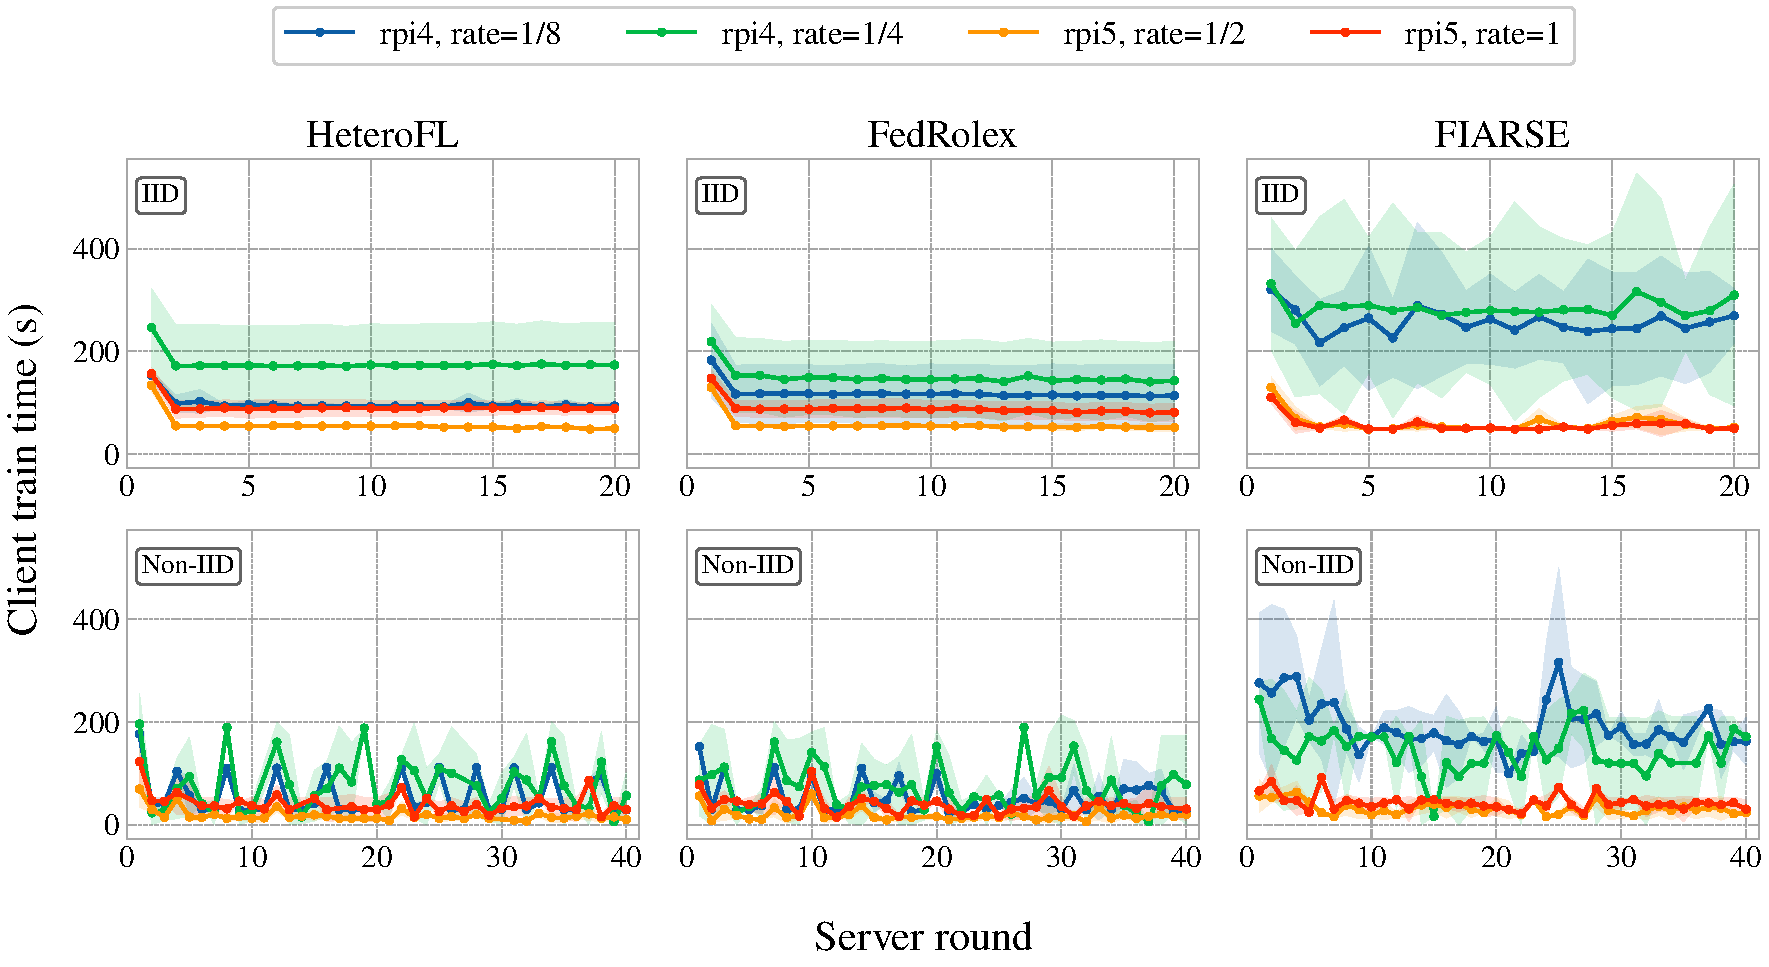
\includegraphics[width=0.98\textwidth]{figures/compute_main_cifar10_seed1340_client_train_time.pdf}
% Notes: rows are IID/non-IID and columns are HeteroFL, FedRolex, and FIARSE.
% Curves show mean update_train_duration_s for each device/rate group per server round.
% Shaded bands show within-group standard deviation across clients.
% IID reruns contain 20 rounds; non-IID reruns contain 40 rounds.
\caption{\textbf{Per-round client training time on CIFAR-10.} Curves split device/rate groups to show which clients gate synchronous rounds.}
\label{fig:compute_cifar10_client_train_time}
\end{figure}

\FloatBarrier
\subsection{Client-Side Submodel Quality}

\paragraph{Setup.}
This subsection addresses \evalqref{C3} by checking whether aggregate quality hides weak client-side submodels. To measure this, the final server model is converted into each rate-specific submodel, sent to every client, and evaluated on that client's local evaluation partition; the figures plot these per-client scores rather than centralized test scores. Figure~\ref{fig:compute_cifar10_seed1340_local_submodel_grid} reports the CIFAR-10 diagnostic, Figure~\ref{fig:compute_california_local_submodel_dist} reports the corresponding California Housing diagnostic, and Appendix~\ref{appendix:fashion_mnist_local_submodel_dist} gives the Fashion-MNIST counterpart.

\begin{figure}[!htbp]
\centering
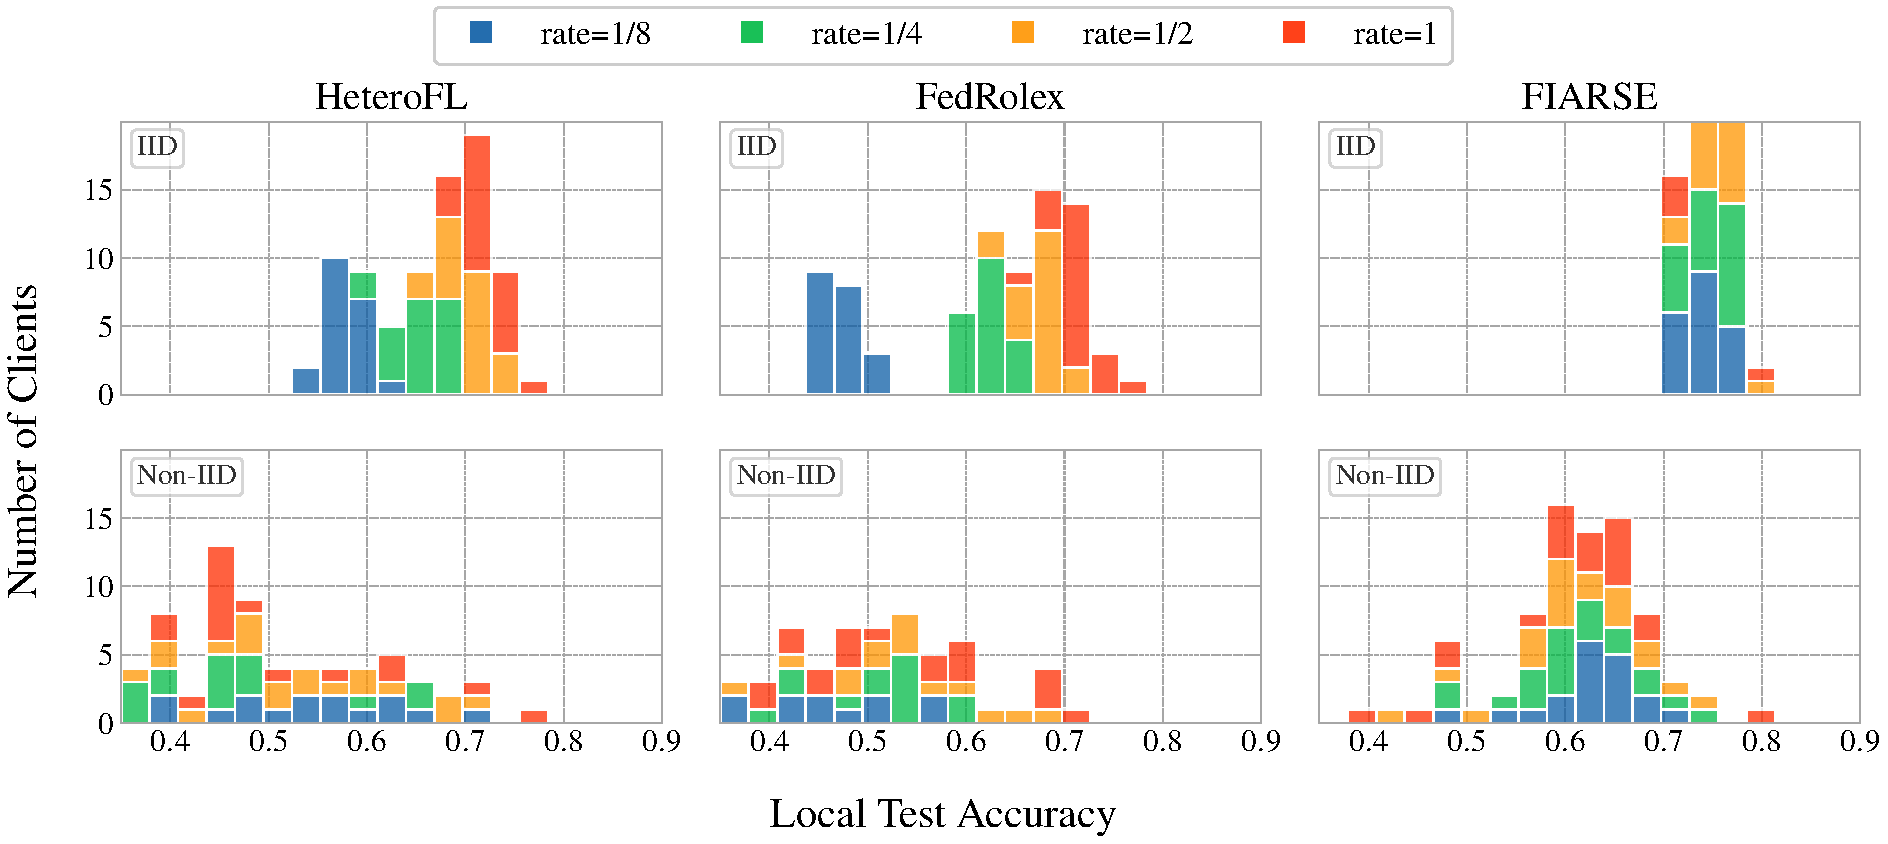
\includegraphics[width=0.98\textwidth]{figures/compute_main_cifar10_seed1340_local_submodel_grid.pdf}
% Notes: rows are IID/non-IID and columns are HeteroFL, FedRolex, and FIARSE.
% Each panel overlays final-round local test accuracy for rates 0.125, 0.25, 0.5, and 1.0 across 20 clients.
% Accuracy is measured on each client's local evaluation partition, not the global test set.
\caption{\textbf{Client-level CIFAR-10 local submodel accuracy distributions.}}
\label{fig:compute_cifar10_seed1340_local_submodel_grid}
\end{figure}

\paragraph{Interpretation.}
In IID CIFAR-10, \texttt{HeteroFL} and \texttt{FedRolex} show a clear rate-based performance gap: lower-rate submodels sit in lower accuracy bands than higher-rate submodels. This is a client-side fairness issue because weaker devices receive systematically weaker deployed models. \texttt{FIARSE} narrows this cross-rate spread, keeping low-rate and high-rate submodels closer together in a higher-accuracy band. Under non-IID data, \texttt{HeteroFL} and \texttt{FedRolex} become more dispersed and left-shifted; \texttt{FIARSE} remains more concentrated around \(60\)--\(70\%\).

\begin{figure}[!htbp]
\centering

\includegraphics[width=0.97\textwidth]{figures/compute_main_california_local_submodel_distributions.pdf}
% Notes: columns are HeteroFL, FedRolex, and FIARSE; rows are IID and non-IID.
% Each panel pools local-client tables from seeds 1337, 1338, and 1339 for that branch.
% The y-axis is clipped at -0.2 for readability; downward markers and annotations report clipped counts and minima.
\caption{\textbf{Client-level California Housing local submodel \(R^2\) distributions.} Panels pool local-client evaluations across seeds.}
\label{fig:compute_california_local_submodel_dist}
\end{figure}

The California Housing IID panels show similar ordering for \texttt{HeteroFL} and \texttt{FedRolex}; \texttt{FIARSE} is already strong at rate \(1/8\). Under non-IID partitioning, central performance remains usable for \texttt{HeteroFL} and \texttt{FIARSE}, but the lower tail becomes heavier and includes clipped negative outliers. \texttt{FedRolex} is especially weak at small rates. Aggregate accuracy and \(R^2\) therefore need to be read with client-level distributions.

\paragraph{Takeaways.}
\begin{itemize}[leftmargin=*, nosep]
  \item Aggregate scores are not enough for submodel FL because each weak client ultimately relies on a rate-specific submodel, not only the global network.
  \item \texttt{FIARSE} gives the most stable CIFAR-10 local-submodel distribution in the inspected reruns, especially under non-IID data.
  \item California Housing shows a residual robustness problem: even when central \(R^2\) is usable, some local submodels have poor tails.
\end{itemize}

\FloatBarrier
\subsection{Client-Capability Mix Sensitivity}

\paragraph{Setup.}
This subsection addresses \evalqref{C4}: whether the compute-heterogeneity result depends on the client-capability mix. The two-rate client-mix sweep varies the proportion of higher-capability clients from \(10\%\) to \(90\%\) while holding two model-rate levels at a time. The three columns in Figure~\ref{fig:compute_fixed_pair_triptych} compare rate \(1\) with rate \(1/4\), rate \(1\) with rate \(1/16\), and rate \(1/4\) with rate \(1/16\).


\paragraph{Interpretation.}
In the \(1\) vs \(1/4\) and \(1\) vs \(1/16\) columns, accuracy improves as the fraction of rate-\(1\) clients increases, but the curves flatten after the early mixture points. \texttt{FIARSE} is strongest when full-capacity clients are present, but dense-kernel execution keeps client training cost high and nearly flat. In the \(1/4\) vs \(1/16\) column, where no full-capacity clients are present, its accuracy advantage mostly disappears. \texttt{HeteroFL} and \texttt{FedRolex} therefore preserve the cleaner realised accuracy--time trade-off.


\begin{figure}[H]
\centering
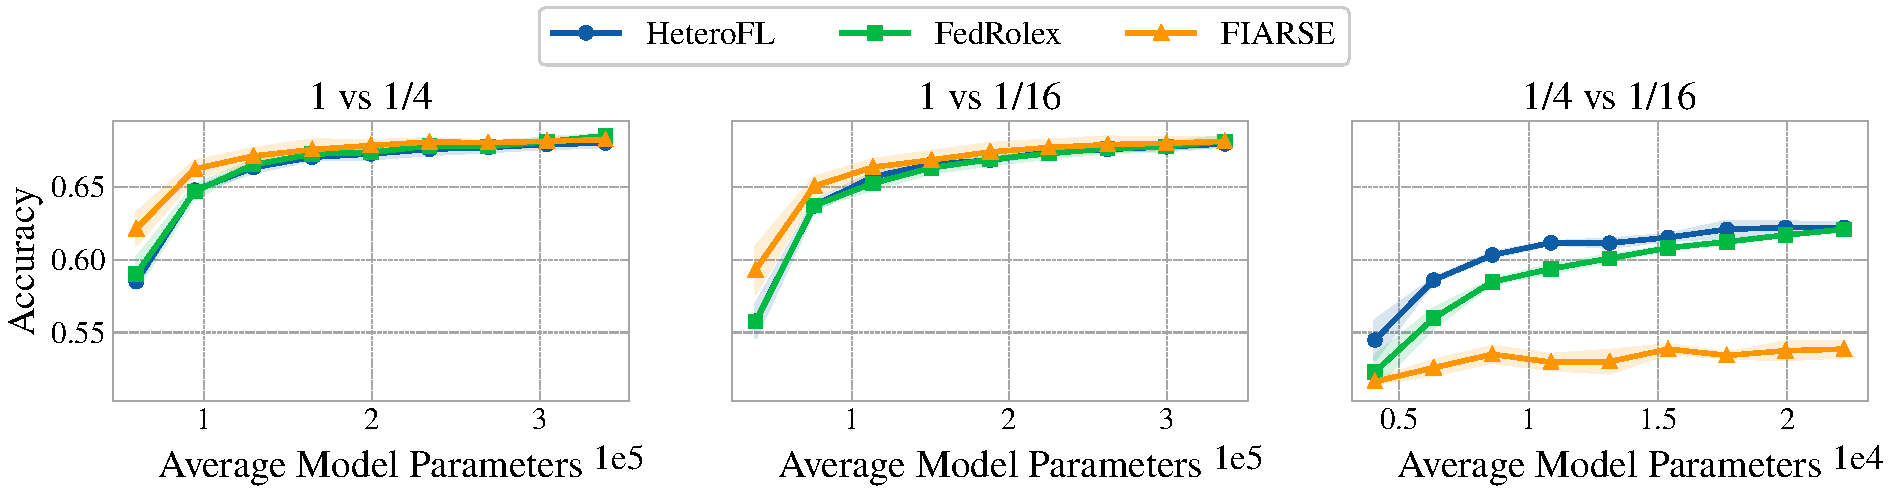
\includegraphics[width=\textwidth]{figures/fixed_pair_interpolation_triptych_methods.pdf}
% Notes: each column varies the proportion of higher-capability clients from 10% to 90%.
% Columns compare model-rate pairs 1 vs 1/4, 1 vs 1/16, and 1/4 vs 1/16.
% The top row reports final global accuracy against average client-side model parameters.
% Points aggregate seeds 1337--1339.
\caption{\textbf{Two-rate client-mix sweep on CIFAR-10 (IID).} Columns vary the client mix between two fixed model-rate levels.}
\label{fig:compute_fixed_pair_triptych}
\end{figure}



\paragraph{Takeaways.}
\begin{itemize}[leftmargin=*, nosep]
  \item The benefit of higher-capability clients is nonlinear: early capacity increases help most.
  \item \texttt{FIARSE}'s quality advantage depends on access to full-capacity clients; sparse-kernel support remains a separate requirement for testing its intended CIFAR-10 runtime benefit.
  \item When only reduced-rate clients are present, \texttt{HeteroFL} and \texttt{FedRolex} give the cleaner realised accuracy--time trade-off.
\end{itemize}

\FloatBarrier
\section{Straggler-Induced Heterogeneity}
\label{sec:eval_network_heterogeneity}

Straggler-induced heterogeneity changes when updates arrive, how stale they are when applied, and how often slower devices influence the server model, as introduced in Section~\ref{sec:background_straggler_heterogeneity}. Previous asynchronous-FL evaluations often simulate staleness or client delay; the cluster runs here measure completion time, staleness, update share, and aggregate weight share directly. The corresponding method family is asynchronous FL, reviewed in Section~\ref{sec:related_async_fl}. This section evaluates asynchronous FL before Section~\ref{sec:eval_async_submodel_fl} combines it with submodel training.

\FloatBarrier
\subsection{Asynchronous FL Across Data and Device Heterogeneity}

\paragraph{Setup.}
This subsection addresses \evalqref{S1}: how asynchronous FL behaves across data regimes and device placements. The CIFAR-10 benchmark crosses \texttt{IID} versus \texttt{non-IID} data with two placements: a homogeneous all-\texttt{rpi5} baseline and a mixed \texttt{rpi4}/\texttt{rpi5} straggler setting. Since all clients train the same model capacity, the placement contrast reflects straggler-induced timing rather than submodel-capacity effects. The methods are \texttt{FedAvg}, \texttt{FedAsync}, \texttt{FedBuff}, and \texttt{FedStaleWeight}, abbreviated as \texttt{FedSW} in compact tables and figures; Appendix~\ref{appendix:evaluation_settings}, Table~\ref{tab:appendix_straggler_settings}, lists their run budgets, buffer sizes, and concurrency settings.

The endpoint is the first server evaluation reaching \(60\%\) accuracy. Time-to-target reports elapsed wall-clock time, while trips to target counts completed client updates to the same threshold; slow-device update share and aggregate-weight share diagnose representation. Figure~\ref{fig:network_main_setup_matrix} summarises the setup and shared stopping rule. Reporting both time and trips separates faster update arrival from better data efficiency, which matters when deployed FL methods are chosen for usable models under a wall-clock budget.

% The mixed-topology rows are completed reruns under the intended placement; earlier submissions had inherited the packed all-\texttt{rpi5} deploy config.

\begin{figure}[!htbp]
\centering
\makebox[\textwidth][c]{%
\hspace*{-0.25cm}%
\begin{tikzpicture}[
  font=\small,
  cell/.style={draw=black!25, rounded corners=2pt, fill=black!3, minimum width=4.35cm, minimum height=1.55cm, align=center},
  header/.style={font=\footnotesize\bfseries, align=center, text=black!75},
  rowlab/.style={font=\footnotesize\bfseries, align=right, text=black!75},
  note/.style={font=\scriptsize, align=center, text=black!70},
  infobox/.style={draw=black!25, rounded corners=2pt, fill=white, minimum width=3.95cm, minimum height=0.8cm, text width=3.55cm, align=center},
  targetbox/.style={draw=paletteGreen!55!black, rounded corners=2pt, fill=paletteGreen!9, minimum width=3.95cm, minimum height=1.0cm, text width=3.55cm, align=center},
  dotrpi5/.style={circle, draw=paletteGreen!80!black, fill=paletteGreen!20, minimum size=4.8mm, inner sep=0pt},
  dotrpi4/.style={circle, draw=paletteOrange!90!black, fill=paletteOrange!22, minimum size=4.8mm, inner sep=0pt},
  arrow/.style={-Latex, line width=0.5pt, draw=black!48}
]
\node[header] at (2.55,4.25) {Control topology\\packed all-\texttt{rpi5}};
\node[header] at (7.25,4.25) {Treatment topology\\mixed \texttt{rpi5}/\texttt{rpi4}};
\node[header, align=left] at (12.05,4.25) {Common run budget\\and endpoint};

\node[cell] (iid5) at (2.55,2.75) {};
\node[cell] (iidm) at (7.25,2.75) {};
\node[cell] (non5) at (2.55,0.45) {};
\node[cell] (nonm) at (7.25,0.45) {};
\node[rowlab] at (-0.3,2.75) {\texttt{IID}\\data};
\node[rowlab] at (-0.4,0.45) {\texttt{non-IID}\\data};

\foreach \n in {iid5,non5} {
  \node[dotrpi5] at ($(\n.center)+(-0.55,0.30)$) {};
  \node[note, text=paletteGreen!70!black] at ($(\n.center)+(0.35,0.30)$) {\(15\times\texttt{rpi5}\)};
  \node[note, text width=3.55cm] at ($(\n.center)+(0,-0.42)$) {homogeneous timing};
}
\foreach \n in {iidm,nonm} {
  \node[dotrpi5] at ($(\n.center)+(-0.70,0.36)$) {};
  \node[note, text=paletteGreen!70!black] at ($(\n.center)+(0.16,0.36)$) {\(10\times\texttt{rpi5}\)};
  \node[dotrpi4] at ($(\n.center)+(-0.70,-0.06)$) {};
  \node[note, text=paletteOrange!90!black] at ($(\n.center)+(0.16,-0.06)$) {\(5\times\texttt{rpi4}\)};
  \node[note, text width=3.55cm] at ($(\n.center)+(0,-0.55)$) {straggler-prone timing};
}

\node[note, infobox]
  (methods) at (12.05,2.75)
  {\texttt{FedAvg}: \(50\) rounds\\
   asynchronous methods: \(100\) server steps};
\node[note, targetbox]
  (target) at (12.05,0.45)
  {first \(60\%\) CIFAR-10 validation accuracy\\
   reported as client trips and wall-clock time};

\draw[arrow] (iidm.east) -- (methods.west);
\draw[arrow] (nonm.east) -- (target.west);
\draw[arrow] (methods.south) -- (target.north);
\end{tikzpicture}%
}
\caption{\textbf{Straggler-induced heterogeneity setup.} Data regime is crossed with topology; the mixed column is the slow-client treatment.}
\label{fig:network_main_setup_matrix}
\end{figure}

% The representation diagnostic is the \texttt{rpi4} update and aggregate-weight share relative to its \(33.3\%\) population share.


\begin{table}[H]
\centering
\scriptsize
% Notes: no-impairment 2x2 matrix over data regime and topology; entries are mean +/- standard deviation over seeds 1337--1339.
% Target-attainment columns report the first point reaching 60% validation accuracy in client trips, wall-clock seconds, and derived throughput.
% Lower is better for trips/time; highlighted target-attainment cells rank the asynchronous methods within each setting.
% Daggered target-attainment cells are lower-bound aggregates: one or more seeds did not reach target, so the final observed client trips or wall-clock time was substituted.
% Diagnostics report accepted-update share, normalized aggregate weight share, and mean staleness in server steps; staleness and throughput cells report means only.
% Daggered values are structural baselines inferred from topology rather than measured asynchronous summaries.
\caption{\textbf{Straggler-induced heterogeneity target-attainment and diagnostics on CIFAR-10.} Columns report trips/time to \(60\%\), update and weight share, and staleness.}
\label{tab:network_main_target_matrix}

\setlength{\tabcolsep}{2.2pt}
\begin{adjustbox}{max width=\textwidth}
\begin{tabular}{@{}lllcccccc@{}}
\toprule
& & & \multicolumn{3}{c}{Target attainment} & \multicolumn{3}{c}{Diagnostics} \\
\cmidrule(lr){4-6}\cmidrule(l){7-9}
Data & Topology & Method
& \makecell{Trips\\to target}
& \makecell{Time to\\target (s)}
& \makecell{Trips/s\\to target}
& \makecell{\texttt{rpi4}\\update \%}
& \makecell{\texttt{rpi4}\\weight \%}
& \makecell{Staleness\\\texttt{rpi4}/\texttt{rpi5}} \\
\midrule
\multirow{8}{*}{IID}
 & \multirow{4}{*}{all-\texttt{rpi5}} & \texttt{FedAvg} & \(195 \pm 0\) & \(651 \pm 34\) & \(0.300\) & \(0.0^\dagger\) & \(0.0^\dagger\) & -- / \(0^\dagger\) \\
 & & \texttt{FedAsync} & \evalbest{\(257 \pm 12\)} & \evalsecond{\(722 \pm 29\)} & \(0.355\) & \(0.0^\dagger\) & \(0.0^\dagger\) & -- / \(13.54\) \\
 & & \texttt{FedBuff} & \(343 \pm 90\) & \(880 \pm 210\) & \(0.390\) & \(0.0^\dagger\) & \(0.0^\dagger\) & -- / \(1.34\) \\
 & & \texttt{FedSW} & \evalsecond{\(273 \pm 6\)} & \evalbest{\(715 \pm 4\)} & \(0.382\) & \(0.0^\dagger\) & \(0.0^\dagger\) & -- / \(1.33\) \\
\cmidrule(lr){2-9}
 & \multirow{4}{*}{mixed} & \texttt{FedAvg} & \(195 \pm 0\) & \(2097 \pm 5\) & \(0.093\) & \(33.3^\dagger\) & \(33.3^\dagger\) & \(0^\dagger\) / \(0^\dagger\) \\
 & & \texttt{FedAsync} & \evalbest{\(137 \pm 6\)} & \evalbest{\(622 \pm 9\)} & \(0.220\) & \(11.9 \pm 0.8\) & \(6.7 \pm 0.7\) & \(35.68\) / \(9.90\) \\
 & & \texttt{FedBuff} & \(387 \pm 15\) & \(1138 \pm 77\) & \(0.340\) & \(13.8 \pm 0.6\) & \(10.1 \pm 0.7\) & \(3.23\) / \(1.05\) \\
 & & \texttt{FedSW} & \evalsecond{\(280 \pm 0\)} & \evalsecond{\(865 \pm 31\)} & \(0.324\) & \(13.8 \pm 0.8\) & \(27.9 \pm 0.7\) & \(3.16\) / \(1.03\) \\
\midrule
\multirow{8}{*}{Non-IID}
 & \multirow{4}{*}{all-\texttt{rpi5}} & \texttt{FedAvg} & \(425 \pm 69\) & \(1320 \pm 205\) & \(0.322\) & \(0.0^\dagger\) & \(0.0^\dagger\) & -- / \(0^\dagger\) \\
 & & \texttt{FedAsync} & \evalsecond{\evalcensored{953 \pm 57}} & \evalcensored{2394 \pm 127} & \(0.398\) & \(0.0^\dagger\) & \(0.0^\dagger\) & -- / \(13.88\) \\
 & & \texttt{FedBuff} & \evalcensored{973 \pm 46} & \evalsecond{\evalcensored{2293 \pm 109}} & \(0.424\) & \(0.0^\dagger\) & \(0.0^\dagger\) & -- / \(1.38\) \\
 & & \texttt{FedSW} & \evalbest{\(620 \pm 85\)} & \evalbest{\(1486 \pm 181\)} & \(0.417\) & \(0.0^\dagger\) & \(0.0^\dagger\) & -- / \(1.37\) \\
\cmidrule(lr){2-9}
 & \multirow{4}{*}{mixed} & \texttt{FedAvg} & \(420 \pm 78\) & \(4043 \pm 437\) & \(0.104\) & \(33.3^\dagger\) & \(33.3^\dagger\) & \(0^\dagger\) / \(0^\dagger\) \\
 & & \texttt{FedAsync} & \evalbest{\(390 \pm 44\)} & \evalbest{\(1264 \pm 111\)} & \(0.309\) & \(12.9 \pm 0.7\) & \(7.5 \pm 0.7\) & \(35.99\) / \(10.33\) \\
 & & \texttt{FedBuff} & \(913 \pm 84\) & \(2388 \pm 128\) & \(0.382\) & \(14.6 \pm 0.7\) & \(10.7 \pm 0.6\) & \(3.27\) / \(1.05\) \\
 & & \texttt{FedSW} & \evalsecond{\(633 \pm 55\)} & \evalsecond{\(1771 \pm 132\)} & \(0.357\) & \(14.6 \pm 0.6\) & \(29.7 \pm 0.3\) & \(3.17\) / \(1.06\) \\
\bottomrule
\end{tabular}
\end{adjustbox}
\par\vspace{0.2em}
{\centering\scriptsize \(\ddagger\) lower-bound aggregate: at least one seed did not reach target.\\\textcolor{evalBestText}{\textbf{Red bold}} text marks the \textbf{best} value and \textcolor{evalSecondText}{blue} text the \textbf{second-best} value among comparable entries. \par}
\end{table}

% \par\vspace{0.5em}
% {\centering\scriptsize \textcolor{evalBestText}{\textbf{Red bold}} text marks the \textbf{best} value and \textcolor{evalSecondText}{blue} text the \textbf{second-best} value among comparable entries.\par}

\paragraph{Interpretation.}
The all-\texttt{rpi5} rows are the negative control: \texttt{FedAvg} reaches the target first in both IID and non-IID settings, while some asynchronous non-IID seeds do not reach target within the trip budget. Mixed topology reverses the wall-clock result. In IID mixed runs, \texttt{FedAsync} reaches target in \(137\pm6\) client trips and \(622\pm9\) s, compared with \(195\pm0\) trips and \(2097\pm5\) s for \texttt{FedAvg}; it is also fastest in non-IID mixed runs. Asynchrony therefore helps under mixed completion times, not simply under non-IID data.


Figure~\ref{fig:network_main_accuracy_combined} shows that asynchronous methods are not consistently more data-efficient. In the all-\texttt{rpi5} panels, \texttt{FedAvg} reaches \(60\%\) with fewer completed trips. The deployment advantage appears only in the wall-clock row: the mixed \texttt{FedAvg} curves are stretched far to the right because synchronous rounds wait for slow devices. \texttt{FedAsync} is fastest, but its speed has a representation cost: \texttt{rpi4} clients provide only about \(12\)--\(13\%\) of accepted updates and roughly \(7\%\) of aggregate weight. \texttt{FedStaleWeight} is slower but raises \texttt{rpi4} aggregate weight to roughly \(28\)--\(30\%\), much closer to the \(5/15\) population share.



\begin{figure}[H]
\centering
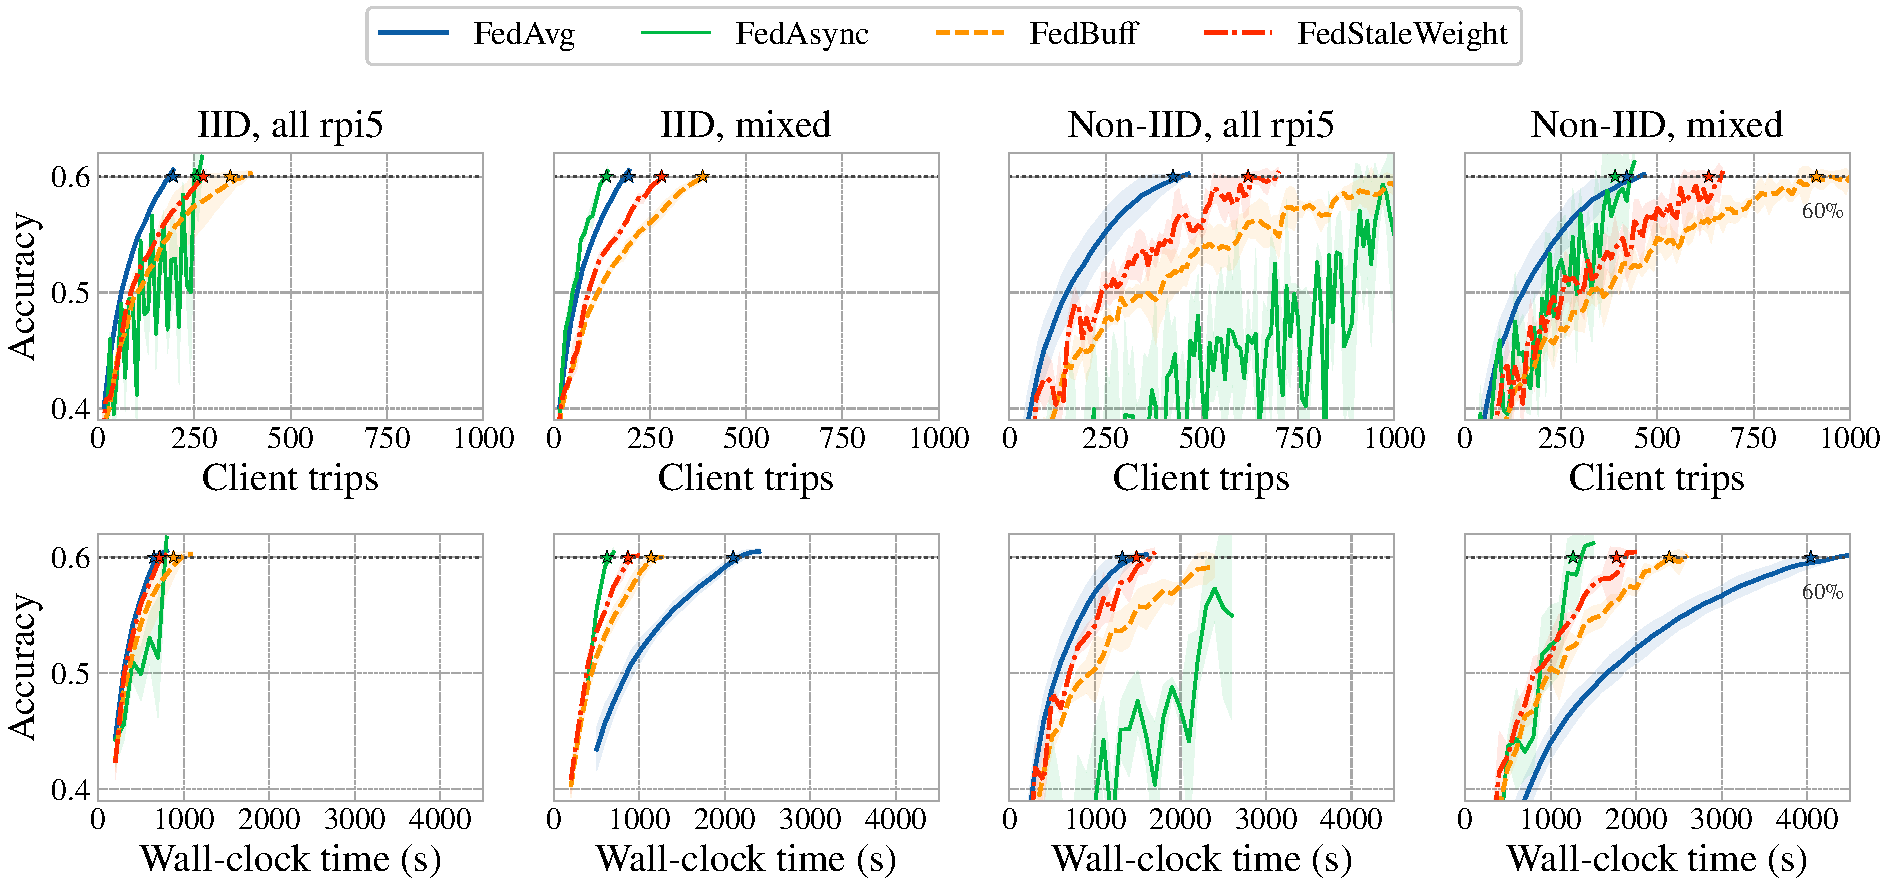
\includegraphics[width=\textwidth]{figures/network_main_accuracy_combined.pdf}
% Notes: top row plots completed client trips; bottom row plots elapsed wall-clock time. Curves show three-seed means with +/- one-standard-deviation bands; the dotted line marks the 60% target.
\caption{\textbf{Straggler-induced heterogeneity accuracy by completed client trips and elapsed wall-clock time.} The dotted horizontal line marks the \(60\%\) target.}
\label{fig:network_main_accuracy_combined}
\end{figure}


\paragraph{Takeaways.}
\begin{itemize}[leftmargin=*, nosep]
  \item In homogeneous all-\texttt{rpi5} runs, synchrony is the better control: \texttt{FedAvg} reaches the target with fewer client trips.
  \item In mixed topology, \texttt{FedAsync} is the fastest wall-clock method, reaching target in \(622\pm9\) s for IID and \(1264\pm111\) s for non-IID.
  \item The speed gain carries a representation cost, while \texttt{FedStaleWeight} trades speed for \texttt{rpi4} aggregate weight closer to population share.
\end{itemize}

\FloatBarrier
\subsection{Network Perturbations: Speed and Representation}

\paragraph{Setup.}
This subsection addresses \evalqref{S2}: how network perturbations affect asynchronous speed and slow-device representation when completion times are mixed. The no-impairment profile is the control; the \texttt{netem} profiles add delay, jitter, loss, and asymmetric bandwidth limits without changing the run config. The experiment also adds \(K=5\) variants for \texttt{FedBuff} and \texttt{FedStaleWeight}, reported in Table~\ref{tab:network_stressor_sweep} as \texttt{FedBuff}\(_5\) and \texttt{FedSW}\(_5\); the main buffered runs use \(K=10\). Smaller buffers test whether buffer-fill latency or update diversity dominates target time under these perturbations.


\begin{figure}[!htbp]
\centering
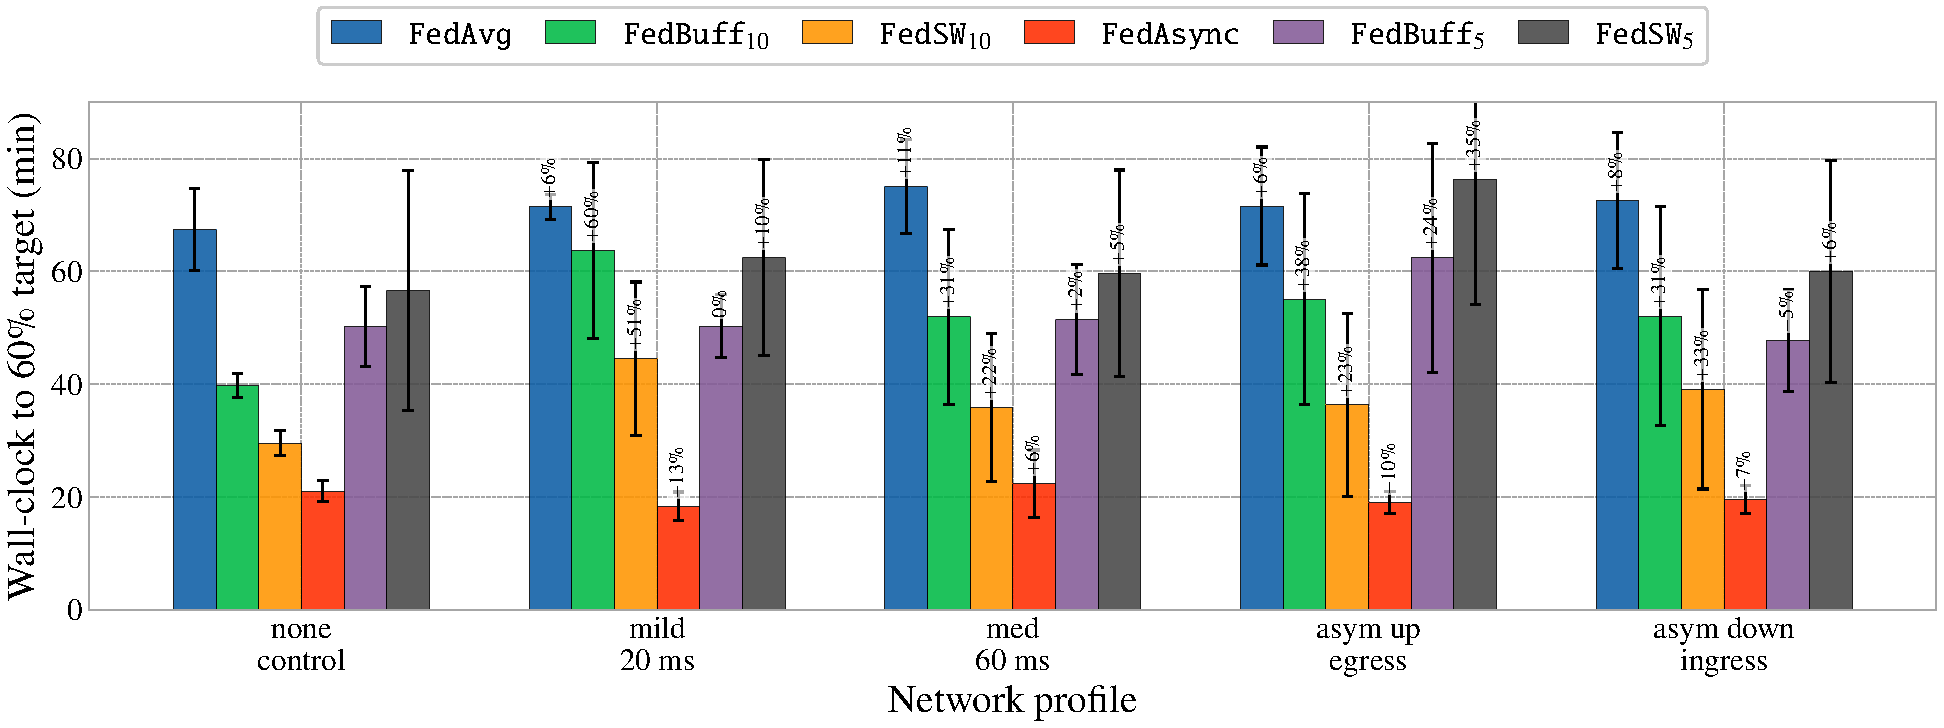
\includegraphics[width=\textwidth]{figures/network_stressor_profile_bars.pdf}
% Notes: bars aggregate seeds 1337--1339. Labels above stressed-profile bars show percentage change from the same method under no added impairment. When a seed did not reach target, its final observed wall-clock time is substituted in the aggregate.
\caption{\textbf{Wall-clock target time across network-stressor profiles.} Labels above stressed-profile bars show percentage change compared to the no-impairment baseline.}
\label{fig:network_stressor_profile_bars}
\end{figure}



\begin{table}[!htbp]
\centering
\scriptsize
% Notes: all runs use 10 rpi5 + 5 rpi4, full local models, and a 60% target.
% Values aggregate seeds 1337, 1338, and 1339.
% The none rows for FedAvg, FedBuff_10, FedSW_10, and FedAsync reuse corresponding main straggler-induced heterogeneity mixed non-IID runs.
% Other rows come from the network_stressor_sweep W&B group.
% Daggered target-attainment cells are lower-bound aggregates: one or more seeds did not reach target, so the final observed client trips or wall-clock time was substituted.
% Diagnostic columns are shown only for asynchronous runs.
\caption{\textbf{Network-stressor sweep on non-IID CIFAR-10 mixed topology.} Rows compare no-impairment and \texttt{netem} profiles, with \(K=10\) and \(K=5\) buffered runs.}
\label{tab:network_stressor_sweep}
\setlength{\tabcolsep}{2.2pt}
\begin{adjustbox}{max width=\textwidth}
\begin{tabular}{@{}p{3.5cm}lrrrrrrr@{}}
\toprule
& & \multicolumn{3}{c}{Target attainment} & \multicolumn{4}{c}{Diagnostics} \\
\cmidrule(lr){3-5}\cmidrule(l){6-9}
\makecell{Profile  /\\Impairment} & Method
& \makecell{Trips\\to target}
& \makecell{Time to\\target (s)}
& \makecell{Final\\acc.}
& \makecell{\texttt{rpi4}\\update \%}
& \makecell{\texttt{rpi4}\\weight \%}
& \makecell{Staleness\\\texttt{rpi4}/\texttt{rpi5}}
& \makecell{Updates/s} \\
\midrule
\multirow{6}{=}{\centering \texttt{none}\\[0.25em]No added impairment}
 & \texttt{FedAvg} & \(420 \pm 78\) & \(4043 \pm 437\) & \(60.2 \pm 0.2\) & -- & -- & -- / -- & -- \\
 & \texttt{FedBuff}\(_{10}\) & \(913 \pm 84\) & \(2388 \pm 128\) & \(60.1 \pm 0.2\) & \(14.6 \pm 0.7\) & \(10.7 \pm 0.6\) & \(3.27\) / \(1.05\) & \(0.382\) \\
 & \texttt{FedSW}\(_{10}\) & \(633 \pm 55\) & \evalsecond{\(1771 \pm 132\)} & \(60.5 \pm 0.2\) & \(14.6 \pm 0.6\) & \(29.7 \pm 0.3\) & \(3.17\) / \(1.06\) & \(0.357\) \\
 & \texttt{FedAsync} & \evalbest{\(390 \pm 44\)} & \evalbest{\(1264 \pm 111\)} & \(61.2 \pm 1.3\) & \(12.9 \pm 0.7\) & \(7.5 \pm 0.7\) & \(35.99\) / \(10.33\) & \(0.308\) \\
 & \texttt{FedBuff}\(_{5}\) & \evalsecond{\(587 \pm 50\)} & \(3014 \pm 423\) & \(60.6 \pm 0.3\) & \(21.4 \pm 1.4\) & \(17.6 \pm 1.7\) & \(4.38\) / \(2.31\) & \(0.198\) \\
 & \texttt{FedSW}\(_{5}\) & \evalcensored{645 \pm 130} & \evalcensored{3396 \pm 1277} & \(53.9 \pm 11.8\) & \(20.5 \pm 1.8\) & \(30.0 \pm 1.1\) & \(4.58\) / \(2.28\) & \(0.199\) \\
\midrule
\multirow{6}{=}{\centering \texttt{mild}\\[0.25em]20 ms, 5 ms jitter\\100 Mbit/s}
 & \texttt{FedAvg} & \(425 \pm 69\) & \(4286 \pm 136\) & \(60.2 \pm 0.1\) & -- & -- & -- / -- & -- \\
 & \texttt{FedBuff}\(_{10}\) & \(900 \pm 104\) & \(3825 \pm 936\) & \(60.4 \pm 0.4\) & \(19.0 \pm 3.4\) & \(15.6 \pm 3.7\) & \(2.54\) / \(1.12\) & \(0.252\) \\
 & \texttt{FedSW}\(_{10}\) & \(617 \pm 40\) & \evalsecond{\(2672 \pm 815\)} & \(60.4 \pm 0.3\) & \(18.9 \pm 4.0\) & \(31.7 \pm 0.7\) & \(2.59\) / \(1.11\) & \(0.253\) \\
 & \texttt{FedAsync} & \evalbest{\(360 \pm 56\)} & \evalbest{\(1101 \pm 152\)} & \(62.2 \pm 1.9\) & \(13.7 \pm 0.7\) & \(8.3 \pm 0.8\) & \(33.49\) / \(10.41\) & \(0.326\) \\
 & \texttt{FedBuff}\(_{5}\) & \evalsecond{\(595 \pm 65\)} & \(3018 \pm 336\) & \(60.3 \pm 0.2\) & \(20.8 \pm 1.9\) & \(17.0 \pm 2.1\) & \(4.47\) / \(2.30\) & \(0.200\) \\
 & \texttt{FedSW}\(_{5}\) & \evalcensored{717 \pm 58} & \evalcensored{3746 \pm 1040} & \(53.5 \pm 8.9\) & \(21.1 \pm 2.4\) & \(30.3 \pm 1.2\) & \(4.48\) / \(2.31\) & \(0.199\) \\
\midrule
\multirow{6}{=}{\centering \texttt{med}\\[0.25em]60 ms, 15 ms jitter\\0.5\% loss, 50 Mbit/s}
 & \texttt{FedAvg} & \(425 \pm 69\) & \(4500 \pm 498\) & \(60.2 \pm 0.1\) & -- & -- & -- / -- & -- \\
 & \texttt{FedBuff}\(_{10}\) & \(923 \pm 121\) & \(3119 \pm 930\) & \(60.4 \pm 0.4\) & \(16.2 \pm 4.1\) & \(12.6 \pm 4.4\) & \(3.05\) / \(1.08\) & \(0.317\) \\
 & \texttt{FedSW}\(_{10}\) & \(620 \pm 69\) & \evalsecond{\(2155 \pm 787\)} & \(60.5 \pm 0.4\) & \(16.3 \pm 4.1\) & \(30.9 \pm 1.0\) & \(3.00\) / \(1.07\) & \(0.313\) \\
 & \texttt{FedAsync} & \evalbest{\(360 \pm 20\)} & \evalbest{\(1341 \pm 359\)} & \(61.0 \pm 0.9\) & \(13.6 \pm 1.2\) & \(8.2 \pm 1.2\) & \(33.96\) / \(10.39\) & \(0.280\) \\
 & \texttt{FedBuff}\(_{5}\) & \evalsecond{\(603 \pm 28\)} & \(3084 \pm 584\) & \(60.4 \pm 0.4\) & \(20.8 \pm 2.1\) & \(17.1 \pm 2.3\) & \(4.49\) / \(2.30\) & \(0.201\) \\
 & \texttt{FedSW}\(_{5}\) & \evalcensored{692 \pm 101} & \evalcensored{3582 \pm 1097} & \(53.2 \pm 7.9\) & \(20.8 \pm 2.3\) & \(29.8 \pm 1.6\) & \(4.52\) / \(2.30\) & \(0.201\) \\
\midrule
\multirow{6}{=}{\centering \makecell[c]{\texttt{asym up}}\\[0.25em]Egress only\\90 ms, 20 ms jitter\\0.5\% loss, 20 Mbit/s}
 & \texttt{FedAvg} & \(420 \pm 65\) & \(4295 \pm 627\) & \(60.1 \pm 0.1\) & -- & -- & -- / -- & -- \\
 & \texttt{FedBuff}\(_{10}\) & \(960 \pm 92\) & \(3306 \pm 1123\) & \(60.2 \pm 0.1\) & \(16.2 \pm 4.2\) & \(12.5 \pm 4.5\) & \(3.04\) / \(1.08\) & \(0.314\) \\
 & \texttt{FedSW}\(_{10}\) & \(617 \pm 55\) & \evalsecond{\(2179 \pm 973\)} & \(60.1 \pm 0.1\) & \(16.0 \pm 4.2\) & \(31.0 \pm 1.5\) & \(3.09\) / \(1.07\) & \(0.315\) \\
 & \texttt{FedAsync} & \evalbest{\(380 \pm 44\)} & \evalbest{\(1141 \pm 115\)} & \(61.2 \pm 1.5\) & \(13.6 \pm 0.8\) & \(8.2 \pm 0.9\) & \(33.88\) / \(10.42\) & \(0.333\) \\
 & \texttt{FedBuff}\(_{5}\) & \evalsecond{\(582 \pm 72\)} & \(3745 \pm 1218\) & \(60.4 \pm 0.3\) & \(21.6 \pm 1.2\) & \(17.8 \pm 1.4\) & \(4.38\) / \(2.30\) & \(0.165\) \\
 & \texttt{FedSW}\(_{5}\) & \evalcensored{735 \pm 26} & \evalcensored{4580 \pm 1329} & \(46.5 \pm 12.2\) & \(21.3 \pm 1.3\) & \(30.6 \pm 0.4\) & \(4.41\) / \(2.32\) & \(0.170\) \\
\midrule
\multirow{6}{=}{\centering \makecell[c]{\texttt{asym down}}\\[0.25em]Ingress only\\90 ms, 20 ms jitter\\0.5\% loss, 20 Mbit/s}
 & \texttt{FedAvg} & \(425 \pm 69\) & \(4351 \pm 722\) & \(60.2 \pm 0.1\) & -- & -- & -- / -- & -- \\
 & \texttt{FedBuff}\(_{10}\) & \(913 \pm 67\) & \(3125 \pm 1163\) & \(60.4 \pm 0.3\) & \(16.6 \pm 4.0\) & \(13.0 \pm 4.2\) & \(2.96\) / \(1.08\) & \(0.319\) \\
 & \texttt{FedSW}\(_{10}\) & \(667 \pm 23\) & \evalsecond{\(2348 \pm 1062\)} & \(60.4 \pm 0.5\) & \(16.5 \pm 4.0\) & \(31.0 \pm 1.0\) & \(2.99\) / \(1.07\) & \(0.317\) \\
 & \texttt{FedAsync} & \evalbest{\(393 \pm 57\)} & \evalbest{\(1173 \pm 152\)} & \(61.9 \pm 2.0\) & \(13.3 \pm 0.5\) & \(8.0 \pm 0.7\) & \(34.56\) / \(10.38\) & \(0.335\) \\
 & \texttt{FedBuff}\(_{5}\) & \evalsecond{\(555 \pm 78\)} & \(2867 \pm 543\) & \(60.4 \pm 0.3\) & \(20.7 \pm 2.0\) & \(16.9 \pm 2.2\) & \(4.51\) / \(2.29\) & \(0.198\) \\
 & \texttt{FedSW}\(_{5}\) & \evalcensored{693 \pm 98} & \evalcensored{3600 \pm 1178} & \(54.8 \pm 6.2\) & \(21.0 \pm 1.7\) & \(30.2 \pm 0.9\) & \(4.51\) / \(2.30\) & \(0.202\) \\
\bottomrule
\end{tabular}
\end{adjustbox}
\par\vspace{0.2em}
{\centering\scriptsize \(\ddagger\) lower-bound aggregate: at least one seed did not reach target. \\ \textcolor{evalBestText}{\textbf{Red bold}} text marks the \textbf{best} value and \textcolor{evalSecondText}{blue} text the \textbf{second-best} value among comparable entries. \par}

\end{table}

\paragraph{Interpretation.}
For synchronous \texttt{FedAvg}, impairment mainly stretches round duration rather than changing optimization progress: the target remains near \(420\)--\(425\) client trips, while mean wall-clock time rises from \(4043\) s with no added impairment to \(4286\)--\(4500\) s under the stressed profiles. The medium profile is the slowest \texttt{FedAvg} case, but the two asymmetric profiles are close to the mild profile, so impairment severity is not captured by latency alone.

\texttt{FedAsync} remains the fastest method in every profile, usually reaching target in \(360\)--\(393\) trips and \(1100\)--\(1340\) s under impairment, but it keeps \texttt{rpi4} aggregate weight near \(8\%\). Its profile-to-profile variation is smaller than the gap to the synchronous baseline, indicating that asynchronous progress is robust to deployment-side network perturbations.

\texttt{FedStaleWeight} with \(K=10\) is the strongest buffered setting: it is slower than \texttt{FedAsync}, but reaches target in every seed and keeps \texttt{rpi4} weight near \(30\%\). The buffered methods are also where the profiles matter most. For \(K=10\), the mild profile is the slowest \texttt{FedBuff} and \texttt{FedStaleWeight} condition, while the medium and asymmetric profiles are closer to each other. This suggests that buffer-fill timing and arrival ordering, not only raw network severity, determine wall-clock target time. Reducing the buffer to \(K=5\) helps \texttt{FedBuff} more reliably than \texttt{FedStaleWeight}; \texttt{FedStaleWeight} with \(K=5\) has large accuracy variance and often fails to reach target under impairment.

Figure~\ref{fig:network_async_participation_staleness} tests the arrival mechanism directly. Across all buffered panels, rows \(11\)--\(15\) are darker and less frequent than rows \(1\)--\(10\), showing that \texttt{rpi4} clients contribute fewer accepted updates and those updates arrive with higher staleness. The \(K=5\) panels have higher absolute staleness for both device classes, while \(K=10\) makes the device-class contrast sharper because most \texttt{rpi5} updates are near-fresh but accepted \texttt{rpi4} updates remain stale. Thus the representation issue is not only how often slow clients arrive, but also how much influence their stale updates receive after aggregation weighting. The corresponding \texttt{FedAsync}-only trace is included as Figure~\ref{fig:appendix_network_fedasync_participation_staleness} in Appendix~\ref{appendix:additional_figures}.



\begin{figure}[H]
\centering

\includegraphics[width=\textwidth]{figures/network_async_participation_staleness.pdf}
% Notes: panels show the first 60 server steps for FedBuff and FedSW with K=5 and K=10.
% Rows 1--10 are rpi5 client slots; rows 11--15 are rpi4 client slots.
% White cells indicate no accepted update; darker cells indicate larger accepted-update staleness.
\caption{\textbf{Accepted asynchronous client updates in mixed non-IID runs.} Rows \(1\)--\(10\) are \texttt{rpi5} client slots and rows \(11\)--\(15\) are \texttt{rpi4}; white cells indicate no accepted update, and darker cells indicate larger accepted-update staleness.}
\label{fig:network_async_participation_staleness}
\end{figure}



\begin{figure}[H]
\centering
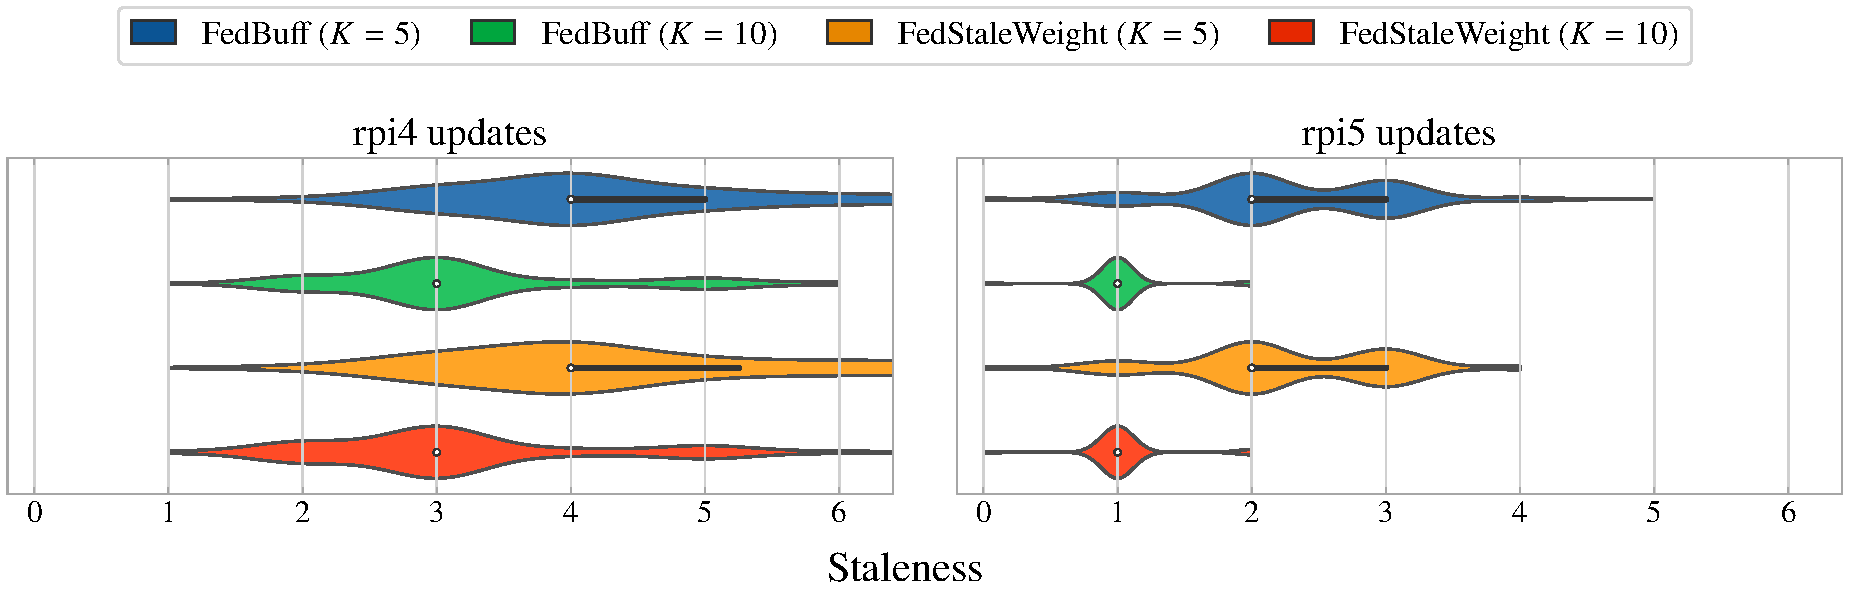
\includegraphics[width=0.98\textwidth]{figures/network_async_staleness_violin.pdf}
% Notes: panels split accepted updates by device class; each violin is one method--buffer setting.
% Inner bars show the interquartile range and the central marker shows the median.
% Distributions pool the first 60 server steps from seeds 1337--1339 for every method--buffer setting.
\caption{\textbf{Accepted-update staleness distributions in mixed non-IID runs.} Violins split accepted updates by device class and buffer setting.}
\label{fig:network_async_staleness_violin}
\end{figure}

Figure~\ref{fig:network_async_staleness_violin} confirms that \texttt{rpi4} updates are systematically staler than \texttt{rpi5} updates. \texttt{FedBuff} and \texttt{FedStaleWeight} have similar staleness distributions at the same \(K\), so their different behaviour comes mainly from the aggregation weights assigned after staleness weighting.


\begin{figure}[H]
\centering
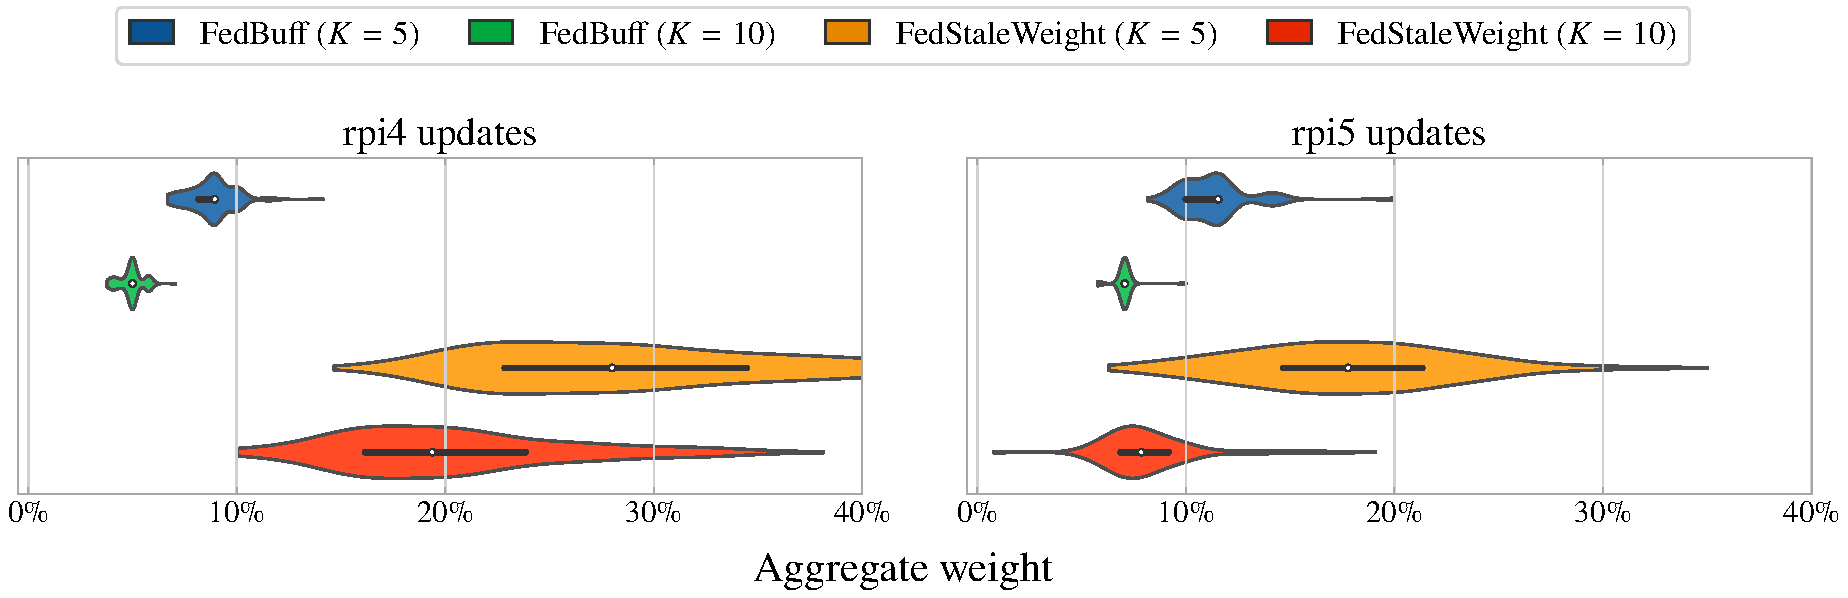
\includegraphics[width=0.98\textwidth]{figures/network_async_weight_violin.pdf}
% Notes: panels split accepted updates by device class.
% The x-axis shows the final aggregation weight assigned after the method-specific staleness rule.
% This separates update arrival frequency from server influence after weighting; seed coverage matches Figure~\ref{fig:network_async_staleness_violin}.
\caption{\textbf{Per-update aggregation weights in mixed non-IID runs.} Violins show the final weight assigned to each accepted update after method-specific staleness weighting, separating update frequency from server influence after weighting.}
\label{fig:network_async_weight_violin}
\end{figure}


Figure~\ref{fig:network_async_weight_violin} shows the difference: \texttt{FedBuff} gives accepted \texttt{rpi4} updates small weights, while \texttt{FedStaleWeight} shifts them into the \(20\)--\(30\%\) range. For \texttt{FedStaleWeight} with \(K=5\), that correction is broad and sometimes over-concentrated on a small set of stale updates, matching its instability in Table~\ref{tab:network_stressor_sweep}.


\paragraph{Takeaways.}
\begin{itemize}[leftmargin=*, nosep]
  \item Network stress mainly increases wall-clock time, but not client-trip count.
  \item \texttt{FedAsync} remains fastest to target under every stress profile, but its \texttt{rpi4} aggregate weight stays near \(8\%\) across profiles.
  \item \texttt{FedStaleWeight} with \(K=10\) is the best buffered representation compromise, while \(K=5\) makes \texttt{FedStaleWeight} unstable in this setting.
\end{itemize}

\FloatBarrier
\subsection{Stale-Aware Weighting Under Device-Correlated Skew}
\label{sec:eval_device_correlated_skew}

\paragraph{Setup.}
This subsection addresses \evalqref{S3} by testing \texttt{FedStaleWeight}'s core motivation: stale-aware weighting should offset slow-client under-representation when slower clients hold different data \parencite{ma2024fedstaleweight}. The ablation ties hardware speed to data: \texttt{rpi4} clients hold CIFAR-10 classes \(0\)--\(4\), while \texttt{rpi5} clients hold classes \(5\)--\(9\). This creates the case targeted by \texttt{FedStaleWeight}: slow clients arrive less often but carry distinct data, so stale-aware reweighting should increase their effective influence.

Table~\ref{tab:network_device_correlated} reports fixed-budget outcomes. \texttt{FedAvg} uses \(50\) rounds with \(15\) clients per round, for \(750\) completed trips; the asynchronous methods use \(150\) server steps with \(K=10\), for \(1500\) completed trips. This gives the asynchronous runs twice as many accepted updates, but \texttt{FedAvg} still takes longer in wall-clock time because each round waits for the slow clients.

\begin{table}[!htbp]
\centering
\scriptsize
% Notes: deployment uses 10 rpi5 + 5 rpi4 with no network impairment and device-correlated data heterogeneity.
% Results report mean +/- standard deviation over seeds 1337--1339.
% Class-group accuracies use seeds 1338--1339 only due to instrumentation availability.
% Accuracy is final centralized test accuracy at the configured budget.
% Class-group accuracies use held-out subsets corresponding to data predominantly assigned to rpi4 and rpi5 clients.
% Diagnostics report rpi4 accepted-update share, rpi4 aggregate-weight share, mean staleness by device, and updates per second; staleness and throughput cells report means only.
% Daggered values are structural synchronous values where update shares match population proportions and staleness is zero.
\caption{\textbf{Device-correlated non-IID fixed-budget ablation on CIFAR-10.} Outcomes are paired with class-group accuracies for labels held mainly by \texttt{rpi4} or \texttt{rpi5} clients.}
\label{tab:network_device_correlated}

\setlength{\tabcolsep}{2.9pt}
\begin{adjustbox}{max width=\textwidth}
\begin{tabular}{@{}lrrrrrrrrrr@{}}
\toprule
& \multicolumn{2}{c}{Fixed-budget outcome}
& \multicolumn{2}{c}{Class-group acc.}
& \multicolumn{2}{c}{\texttt{rpi4}}
& \multicolumn{2}{c}{Staleness}
& \\
\cmidrule(lr){2-3}
\cmidrule(lr){4-5}
\cmidrule(lr){6-7}
\cmidrule(lr){8-9}
Method
& \makecell{Wall\\clock (s)}
& \makecell{Final\\acc.}
& \makecell{\texttt{rpi4}\\held}
& \makecell{\texttt{rpi5}\\held}
& \makecell{update\\\%}
& \makecell{weight\\\%}
& \texttt{rpi4}
& \texttt{rpi5}
& \makecell{Updates/s} \\
\midrule
\texttt{FedAvg} & 8915 $\pm$ 596 & 40.8 $\pm$ 1.6 & 5.6 $\pm$ 2.6 & 75.8 $\pm$ 2.3 & 33.3$^\dagger$ & 33.3$^\dagger$ & 0$^\dagger$ & 0$^\dagger$ & 0.084 \\
\texttt{FedBuff} & \evalsecond{5840 $\pm$ 1613} & 40.8 $\pm$ 1.8 & 0.0 $\pm$ 0.0 & 80.6 $\pm$ 5.7 & 15.9 $\pm$ 2.5 & 12.2 $\pm$ 2.7 & 3.02 & 1.09 & 0.275 \\
\texttt{FedStaleWeight} & \evalbest{5813 $\pm$ 1588} & \evalbest{45.9 $\pm$ 1.3} & 12.9 $\pm$ 7.3 & 79.7 $\pm$ 5.9 & 15.7 $\pm$ 2.8 & 31.0 $\pm$ 0.3 & 3.08 & 1.09 & 0.276 \\
\texttt{FedAsync} & 7070 $\pm$ 19 & \evalsecond{43.0 $\pm$ 1.5} & 0.0 $\pm$ 0.0 & 86.1 $\pm$ 3.0 & 17.5 $\pm$ 0.1 & 11.9 $\pm$ 0.1 & 27.33 & 11.07 & 0.213 \\
\bottomrule
\end{tabular}
\end{adjustbox}
\end{table}

\paragraph{Interpretation.}
Despite being given twice as many completed trips, the asynchronous methods finish in less wall-clock time than \texttt{FedAvg}; device-correlated skew nevertheless remains hard. \texttt{FedStaleWeight} gives the best global accuracy at \(45.9 \pm 1.3\%\) and is the only method to noticeably improve the \texttt{rpi4}-held group, reaching \(12.9 \pm 7.3\%\). Even so, the device gap remains large: the \texttt{rpi5}-held group reaches roughly \(76\)--\(86\%\) accuracy, while the \texttt{rpi4}-held group is \(5.6 \pm 2.6\%\) for \texttt{FedAvg} and \(0.0 \pm 0.0\%\) for both \texttt{FedBuff} and \texttt{FedAsync}.

\begin{figure}[!htbp]
\centering
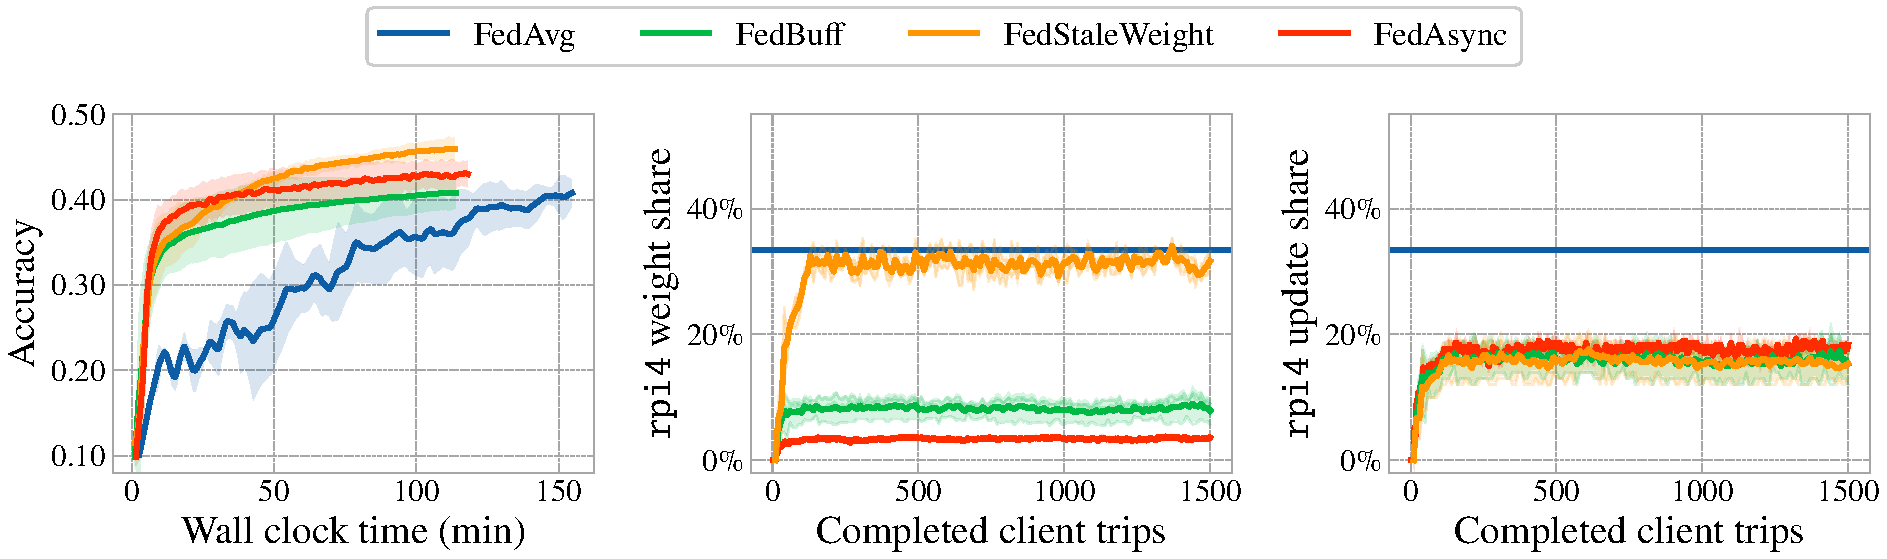
\includegraphics[width=\textwidth]{figures/network_device_correlated.pdf}
% Notes: the left panel shows three-seed mean centralized accuracy against wall-clock time with +/- one-standard-deviation bands.
% The middle and right panels show rpi4 weight and accepted-update shares over completed client trips.
% Faint traces are per-seed rolling means over a matched client-trip window; solid traces are their mean; shaded bands show +/- one standard deviation.
% The horizontal reference line in the share panels marks the structural rpi4 population share 5/15.
\caption{\textbf{Device-correlated non-IID accuracy and device-share diagnostics.} Traces separate slow-device update frequency from aggregate influence.}
\label{fig:network_device_correlated}
\end{figure}

Figure~\ref{fig:network_device_correlated} separates update frequency from aggregate influence. All asynchronous methods receive an \texttt{rpi4} update share below the \(33.3\%\) population share. \texttt{FedStaleWeight} raises \texttt{rpi4} aggregate weight close to population share and improves global accuracy, but it does not increase slow-client arrival frequency or recover strong \texttt{rpi4}-held class accuracy.

\paragraph{Takeaways.}
\begin{itemize}[leftmargin=*, nosep]
  \item Device-correlated skew is the hardest setting in this straggler-induced study: global accuracy remains low and the \texttt{rpi4}-held class group is poorly learned.
  \item \texttt{FedStaleWeight} improves global accuracy and slow-device aggregate influence, but the \texttt{rpi4}-held class group remains weak.
  \item Weighting stale updates helps representation but cannot replace more frequent slow-client participation or data-aware correction.
\end{itemize}

\FloatBarrier
\section{Asynchronous Submodel Federated Learning}
\label{sec:eval_async_submodel_fl}

The previous sections evaluate synchronous submodel training and standard asynchronous training separately. This section combines them and tests \texttt{FedCover} from Section~\ref{sec:fedcover_impl}, using accepted asynchronous submodel buffers to measure parameter coverage during aggregation.

\FloatBarrier
\subsection{Feasibility Across Tasks and Data Regimes}

\paragraph{Setup.}
This subsection addresses \evalqref{A1}: whether asynchronous submodel FL is feasible across tasks and data regimes. The comparison uses the same \(20\)-node mixed deployment and nested \texttt{HeteroFL} rate assignment as the compute benchmark. Methods are synchronous \texttt{HeteroFL}, coverage-disabled asynchronous \texttt{HeteroFL} labelled \texttt{Async-HeteroFL}, \texttt{FedCover}, and \texttt{FedBuff}; \texttt{Async-HeteroFL} is the direct buffered composition isolating \texttt{FedCover}'s coverage correction. Unlike workload-adaptive approaches such as \texttt{TimelyFL}, this experiment keeps the nested rate assignment fixed and tests aggregation-side coverage. Appendix~\ref{appendix:evaluation_settings}, Table~\ref{tab:appendix_fedcover_settings}, lists run settings. All \texttt{FedCover} rows use \(\kappa_{\max}=3\), so sweep differences reflect \(\gamma\), not the correction cap.

\paragraph{Interpretation.}
The table shows that the combined setting is operationally feasible rather than merely a conceptual composition. Asynchronous submodel variants reach target in all CIFAR-10 runs, including the non-IID regime where synchronous \texttt{HeteroFL} reaches the \(60\%\) target for only \(2/3\) seeds. Fashion-MNIST shows the same feasibility pattern under IID data and a harder non-IID case: every cap-matched \texttt{FedCover} setting reaches the \(75\%\) target for every seed, while the synchronous and coverage-disabled baselines each have at least one censored seed. \texttt{FedBuff} is retained as an asynchronous reference, but it is not capacity-matched to the submodel methods and is therefore unranked.


\paragraph{Takeaways.}
\begin{itemize}[leftmargin=*, nosep]
  \item Asynchronous submodel FL is feasible across the CIFAR-10 and Fashion-MNIST settings.
  \item Non-IID Fashion-MNIST is the hardest feasibility case, with censored seeds for the synchronous and coverage-disabled baselines.
  \item \texttt{Async-HeteroFL} is the controlled coverage-disabled baseline for the next subsection; \texttt{FedBuff} remains contextual because it is not capacity-matched.
\end{itemize}

\begin{table}[H]
\centering
\scriptsize
\renewcommand{\arraystretch}{1.02}
\setlength{\tabcolsep}{2pt}
% Notes: values are mean +/- standard deviation over seeds 1337--1339.
% The target is first centralized accuracy >= the task/data target stated in the surrounding paragraph.
% Daggered trip/time cells are lower-bound aggregates: one or more seeds did not reach target, so the final observed run point was substituted.
% Post-warm-up time subtracts the first 20 completed client trips: one synchronous HeteroFL round or five async buffered server steps.
% rpi4 weight share is aggregate server weight assigned to rpi4 updates; synchronous HeteroFL has the structural 50% share.
% Coverage gain is the mean FedCover multiplicative correction; the daggered async-HeteroFL value is the disabled-correction baseline.
% All FedCover rows use kappa_max = 3; gamma is the swept coverage-power parameter.
% FedBuff is a higher-capacity full-model asynchronous reference, not a capacity-matched baseline.
\caption{\textbf{Asynchronous submodel FL with coverage-aware aggregation.} Target metrics use task-specific IID/non-IID thresholds; all \texttt{FedCover} rows use \(\kappa_{\max}=3\).}  
\label{tab:fedcover_async_submodel}
\begin{adjustbox}{max width=\textwidth}
\begin{tabular}{@{}lllccccc@{}}
\toprule
Task & Data & Method & \makecell{Trips\\to target} & \makecell{Time to\\target (min)} & \makecell{Post-warm-up\\target (min)} & \makecell{\texttt{rpi4}\\weight (\%)} & \makecell{Coverage\\gain} \\
\midrule
\multirow{14}{*}{\makecell[l]{CIFAR-10}} & \multirow{7}{*}{IID} & \texttt{FedBuff}\(^*\) & \(120\pm0\) & \(35.7\pm7.5\) & \(19.8\pm0.3\) & \(34.3\pm0.7\) & -- \\
 &  & \texttt{HeteroFL} & \(193\pm12\) & \(24.2\pm2.9\) & \(18.3\pm2.7\) & \(50.0\pm0.0\) & -- \\
 &  & \texttt{Async-HeteroFL} & \(227\pm12\) & \(33.9\pm16.0\) & \(18.4\pm1.8\) & \(44.5\pm0.3\) & \(1.00^\dagger\) \\
 &  & \texttt{FedCover} \((\gamma=0.25)\) & \(193\pm12\) & \(19.9\pm0.6\) & \(15.2\pm1.4\) & \(44.9\pm0.5\) & \(1.23\pm0.11\) \\
 &  & \texttt{FedCover} \((\gamma=0.5)\) & \(167\pm12\) & \(17.1\pm0.9\) & \(12.7\pm1.1\) & \(44.0\pm2.8\) & \(2.03\pm0.56\) \\
 &  & \texttt{FedCover} \((\gamma=1.0)\) & \evalsecond{\(133\pm12\)} & \evalsecond{\(13.8\pm0.6\)} & \evalsecond{\(9.7\pm0.9\)} & \(43.6\pm1.3\) & \(2.65\pm0.06\) \\
 &  & \texttt{FedCover} \((\gamma=1.5)\) & \evalbest{\(127\pm12\)} & \evalbest{\(13.7\pm2.1\)} & \evalbest{\(9.3\pm1.1\)} & \(42.6\pm0.6\) & \(2.73\pm0.17\) \\
\cmidrule(l){2-8}
 & \multirow{7}{*}{Non-IID} & \texttt{FedBuff}\(^*\) & \(133\pm12\) & \(30.2\pm3.3\) & \(19.1\pm3.5\) & \(32.6\pm1.4\) & -- \\
 &  & \texttt{HeteroFL} & \evalcensored{420\pm80} & \evalcensored{51.6\pm19.2} & \evalcensored{39.3\pm12.5} & \(50.0\pm0.0\) & -- \\
 &  & \texttt{Async-HeteroFL} & \(400\pm35\) & \(38.2\pm9.1\) & \(29.2\pm3.9\) & \(45.0\pm2.3\) & \(1.00^\dagger\) \\
 &  & \texttt{FedCover} \((\gamma=0.25)\) & \(380\pm151\) & \(31.3\pm11.4\) & \(27.5\pm11.4\) & \(43.6\pm1.1\) & \(1.27\pm0.08\) \\
 &  & \texttt{FedCover} \((\gamma=0.5)\) & \(273\pm31\) & \(23.1\pm2.7\) & \(19.4\pm2.7\) & \(45.0\pm1.5\) & \(2.22\pm0.36\) \\
 &  & \texttt{FedCover} \((\gamma=1.0)\) & \evalsecond{\(220\pm92\)} & \evalsecond{\(18.8\pm7.1\)} & \evalsecond{\(15.3\pm7.1\)} & \(43.3\pm1.4\) & \(2.81\pm0.10\) \\
 &  & \texttt{FedCover} \((\gamma=1.5)\) & \evalbest{\(187\pm12\)} & \evalbest{\(16.3\pm0.3\)} & \evalbest{\(12.8\pm0.4\)} & \(44.2\pm2.6\) & \(2.91\pm0.08\) \\
\midrule
\multirow{14}{*}{\makecell[l]{Fashion\\MNIST}} & \multirow{7}{*}{IID} & \texttt{FedBuff}\(^*\) & \(160\pm20\) & \(7.2\pm0.7\) & \(5.3\pm0.7\) & \(36.1\pm0.8\) & -- \\
 &  & \texttt{HeteroFL} & \(273\pm23\) & \(12.9\pm1.1\) & \(12.0\pm1.1\) & \(50.0\pm0.0\) & -- \\
 &  & \texttt{Async-HeteroFL} & \(347\pm42\) & \(11.8\pm1.4\) & \(10.1\pm1.4\) & \(41.2\pm0.6\) & \(1.00^\dagger\) \\
 &  & \texttt{FedCover} \((\gamma=0.25)\) & \(307\pm12\) & \(10.6\pm0.4\) & \(8.9\pm0.4\) & \(42.1\pm0.8\) & \(1.42\pm0.10\) \\
 &  & \texttt{FedCover} \((\gamma=0.5)\) & \(240\pm20\) & \(8.6\pm0.7\) & \(6.9\pm0.7\) & \(40.3\pm1.5\) & \(1.99\pm0.51\) \\
 &  & \texttt{FedCover} \((\gamma=1.0)\) & \evalsecond{\(167\pm12\)} & \evalsecond{\(6.2\pm0.3\)} & \evalsecond{\(4.5\pm0.3\)} & \(39.4\pm0.4\) & \(2.93\pm0.04\) \\
 &  & \texttt{FedCover} \((\gamma=1.5)\) & \evalbest{\(160\pm20\)} & \evalbest{\(6.0\pm0.7\)} & \evalbest{\(4.4\pm0.6\)} & \(38.6\pm0.6\) & \(2.93\pm0.06\) \\
\cmidrule(l){2-8}
 & \multirow{7}{*}{Non-IID} & \texttt{FedBuff}\(^*\) & \(180\pm40\) & \(7.7\pm1.5\) & \(5.9\pm1.5\) & \(35.6\pm3.0\) & -- \\
 &  & \texttt{HeteroFL} & \evalcensored{473\pm46} & \evalcensored{22.6\pm2.8} & \evalcensored{21.8\pm2.9} & \(50.0\pm0.0\) & -- \\
 &  & \texttt{Async-HeteroFL} & \evalcensored{613\pm167} & \evalcensored{20.5\pm6.4} & \evalcensored{18.8\pm6.4} & \(38.7\pm1.5\) & \(1.00^\dagger\) \\
 &  & \texttt{FedCover} \((\gamma=0.25)\) & \(607\pm214\) & \(19.4\pm6.3\) & \(17.8\pm6.2\) & \(39.3\pm2.3\) & \(1.45\pm0.11\) \\
 &  & \texttt{FedCover} \((\gamma=0.5)\) & \(467\pm76\) & \evalsecond{\(15.2\pm2.3\)} & \(13.5\pm2.3\) & \(39.8\pm1.3\) & \(1.71\pm0.12\) \\
 &  & \texttt{FedCover} \((\gamma=1.0)\) & \evalsecond{\(460\pm296\)} & \(15.5\pm9.9\) & \evalsecond{\(13.4\pm9.0\)} & \(39.9\pm2.9\) & \(2.46\pm0.53\) \\
 &  & \texttt{FedCover} \((\gamma=1.5)\) & \evalbest{\(327\pm76\)} & \evalbest{\(11.0\pm2.3\)} & \evalbest{\(9.3\pm2.3\)} & \(39.9\pm1.0\) & \(2.90\pm0.12\) \\
\bottomrule
\end{tabular}
\end{adjustbox}
\par\vspace{0.2em}
{\centering\scriptsize \(\ddagger\) lower-bound aggregate: at least one seed did not reach target. \\ \(^*\)\texttt{FedBuff} is a full-model, higher-capacity asynchronous baseline reference and is thus unranked.\par}
\end{table}


\FloatBarrier
\subsection{Coverage-Aware Aggregation with FedCover}
\label{sec:eval_coverage_mismatch}

\paragraph{Setup.}
Building on the same runs reported in Table~\ref{tab:fedcover_async_submodel}, this subsection addresses \evalqref{A2}: whether \texttt{FedCover}'s coverage correction improves asynchronous submodel FL. The capacity-matched comparison is synchronous \texttt{HeteroFL}, coverage-disabled asynchronous \texttt{HeteroFL}, and \texttt{FedCover} across \(\gamma\) values. \texttt{FedBuff} remains an asynchronous reference rather than a capacity-matched baseline.

\paragraph{Interpretation.}
On CIFAR-10 IID, \texttt{FedCover} gives the clearest target-time improvement among capacity-matched methods: \(\gamma=1.5\) reduces mean time to target from \(24.2\) minutes for synchronous \texttt{HeteroFL} and \(33.9\) minutes for coverage-disabled asynchronous \texttt{HeteroFL} to \(13.7\) minutes, with the lowest trip count and post-warm-up target time. With the cap fixed, \(\gamma=1.0\) is now close behind at \(13.8\) minutes and \(9.7\) post-warm-up minutes. The non-IID setting strengthens the need for the larger correction: \(\gamma=1.5\) reaches the \(60\%\) target in \(16.3\) minutes, compared with \(38.2\) minutes for the coverage-disabled asynchronous baseline and \(18.8\) minutes for \(\gamma=1.0\).

Fashion-MNIST repeats the same main pattern on a second image task. In IID, \(\gamma=1.5\) reaches the \(80\%\) target in \(6.0\) minutes and reduces post-warm-up time to \(4.4\) minutes, only slightly ahead of \(\gamma=1.0\). In non-IID, \(\gamma=1.5\) is again the strongest target-time setting; \(\gamma=1.0\) has the second-best post-warm-up mean, while \(\gamma=0.5\) is marginally second on total target time.

Figure~\ref{fig:fedcover_post_warmup_speedup} makes the post-warm-up pattern clearer. Every \(\gamma\) setting has positive mean speedup over coverage-disabled \texttt{Async-HeteroFL} after warm-up. The IID panels show the cleanest trend: larger \(\gamma\) and larger observed coverage gain \(\bar{\kappa}\) give consistent speedup, with \(\gamma=1.0\) close to \(\gamma=1.5\). The non-IID panels are more seed-sensitive for weaker corrections, but \(\gamma=1.5\) gives the largest average speedup in both tasks, reaching roughly \(56\%\) on CIFAR-10 and \(48\%\) on Fashion-MNIST. This supports the interpretation that \texttt{FedCover} is compensating for under-covered parameter blocks after warm-up, while also showing that the strongest correction matters most under data skew. Its \texttt{rpi4} aggregate weight remains close to the coverage-disabled asynchronous baseline, so the improvement comes from coverage-aware aggregation rather than simply increasing slow-device aggregate weight.

\begin{figure}[!htbp]
\centering
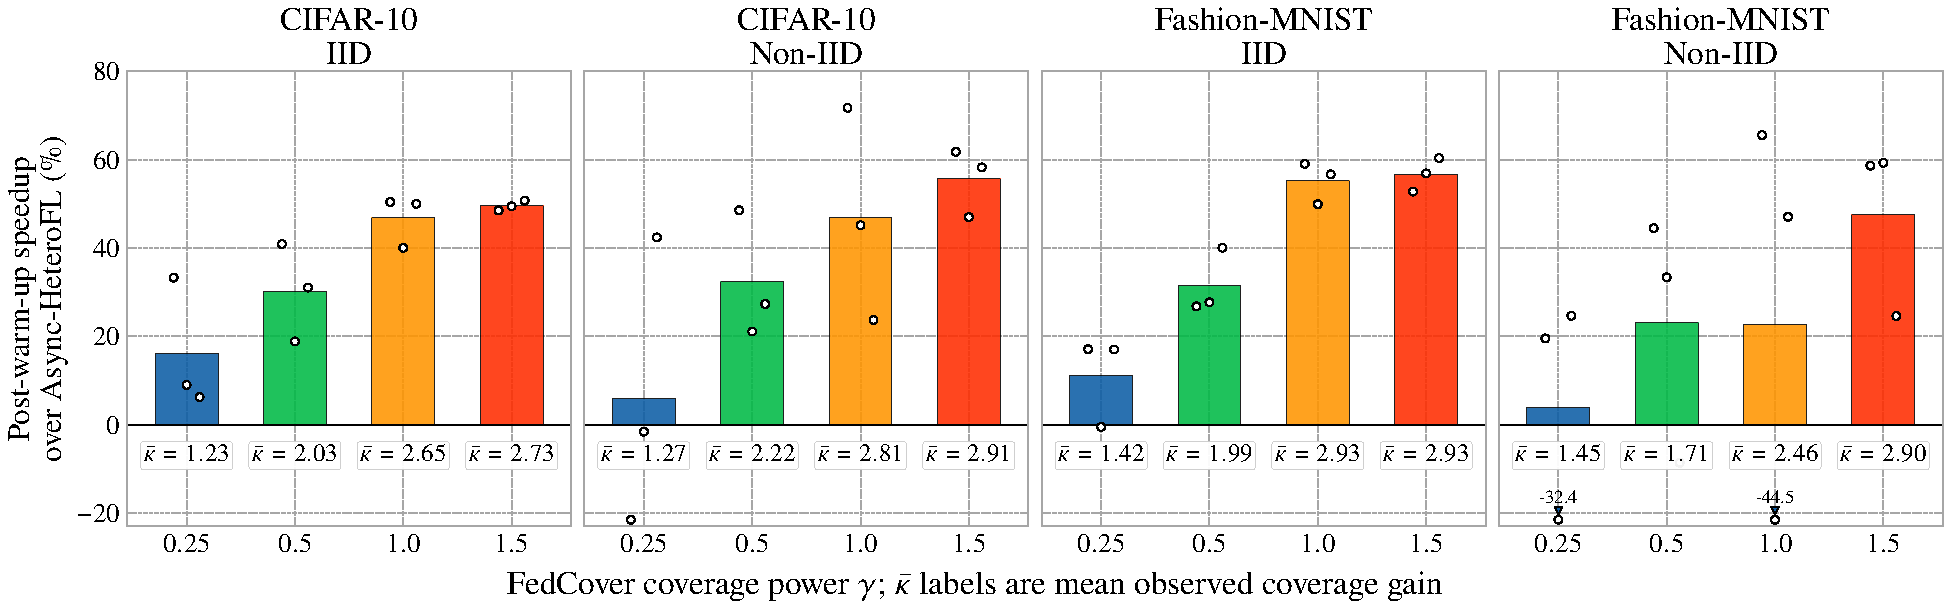
\includegraphics[width=\textwidth]{figures/fedcover_post_warmup_speedup.pdf}
\caption{\textbf{Post-warm-up speedup from coverage-aware aggregation.} Bars show mean paired-seed speedup over coverage-disabled \texttt{Async-HeteroFL}; open circles show seeds.}
\label{fig:fedcover_post_warmup_speedup}
\end{figure}

\paragraph{Takeaways.}

\begin{itemize}[leftmargin=*, nosep]
  \item \texttt{FedCover} improves the coverage-disabled \texttt{Async-HeteroFL} baseline across all task--regime pairs, especially in target time and post-warm-up time.
  \item With \(\kappa_{\max}\) fixed, \(\gamma=1.0\) nearly matches \(\gamma=1.5\) on IID data, while \(\gamma=1.5\) is strongest under non-IID data.
  \item The gains are not explained by slow-device reweighting: \texttt{rpi4} aggregate weight stays close to \texttt{Async-HeteroFL}, so the improvement is consistent with correcting under-covered parameter blocks.
\end{itemize}

\FloatBarrier
% \subsection{Platform and Reproducibility Evidence}

% The execution path is also part of the evaluated contribution. The headline compute-heterogeneity and straggler-induced heterogeneity evaluations were launched through the same \texttt{fedctl submit} path: a Flower run config defined the learning problem and method parameters, while a deploy config defined placement, device type, oversubscription, and optional \texttt{netem} impairment. This split is what made the controls above practical: the network-stressor sweep changed the deployment-side impairment while preserving the learning configuration, and the compute-heterogeneity experiments changed model-rate assignment while preserving the mixed rack.

% Each submission preserved the reconstructed request, run config, deploy config, Nomad jobs, logs, W\&B metrics, and result artifacts. This matters scientifically because failed, censored, or rerun experiments remain inspectable rather than disappearing as terminal cluster jobs. The corrected mixed-topology network reruns are the clearest example: the stored submission state made the placement error visible and allowed the affected runs to be repeated under the intended mixed topology.

% Overall, the evaluation supports three conclusions. First, submodel FL is useful on the live Raspberry Pi rack when local compute is a real bottleneck, but the best method depends on whether the objective is quality or speed: \texttt{FIARSE} gives stronger submodel quality, while \texttt{HeteroFL} and \texttt{FedRolex} give clearer wall-clock savings. Second, asynchronous coordination is not uniformly better than synchronous training; it helps mainly when completion times are heterogeneous, and its advantage is primarily a wall-clock effect rather than a universal reduction in client trips. Third, stale-aware weighting can restore the aggregate influence of slow devices, but it does not make those devices participate more often. Device-correlated data skew therefore remains difficult and is not solved by weighting alone.
